\graphicspath{{surfaces/asy/}}

\section{Surfaces}\label{chap:surfaces}

\subsection{Regular Parametrized Surfaces}\label{sec:regularsurfaces}

We approach surfaces in $\E^3$ similarly to how we considered curves; a parametrized surface is a \emph{function} $\vx:U\to\E^3$ where $U$ is some open subset of the plane $\R^2$. Our main purpose is to develop and measure the \emph{curvature} of a surface in terms of the parametrizing function $\vx$.\medbreak


Our primary definition should mostly be familiar from elementary multivariable calculus.

\begin{defn}{}{surface}
	A \emph{(smooth local) surface} is the range $S=\vx(U)$ of a smooth function $\vx:U\to\E^3$, where $U$ is a connected open subset of $\R^2$.\smallbreak
	Given co-ordinates $u,v$ on $U$, the \emph{co-ordinate tangent vector fields} are the partial derivatives $\vx_u=\partials[\vx]{u}$ and $\vx_v=\partials[\vx]{v}$.\smallbreak
	The \emph{exterior derivative} or \emph{differential} of the surface is the vector-valued 1-form $\dvx=\vx_u\,\du+\vx_v\,\dv$.\smallbreak
	A surface is \emph{regular} at $P=\vx(p)$ if the tangent vectors $\vx_u(p)$ and $\vx_v(p)$ are \emph{linearly independent}: otherwise said, at $P$, the surface has a well-defined
	\begin{quote}
		\emph{Tangent plane} \ $T_PS=\Span\bigl\{\vx_u(p),\vx_v(p)\bigr\}$ (a 2-dim subspace of $T_P\E^3$), \ and \smallbreak
		\emph{Unit normal vector} \ $\vn(p)=\dfrac{\vx_u(p)\times\vx_v(p)}{\Nm{\vx_u(p)\times\vx_v(p)}} \in T_P\E^3$
	\end{quote} 
	$S$ is \emph{regular} if it is regular everywhere. An \emph{orientation} is a smooth choice of \emph{unit normal vector field} $\vn$.
\end{defn}

The \emph{Möbius strip} (Exercise \ref{exs:mobius}) shows that not every surface is orientable!\par
For brevity, we will often refer to the parametrizing function $\vx$ as the surface, though many different parametrizations will exist! A general surface typically needs to be parametrized by several overlapping functions $\vx_1,\vx_2,\ldots$. Our definition is \emph{local} since there is only one $\vx$.


\begin{center}\phantomsection\label{sec:map}
	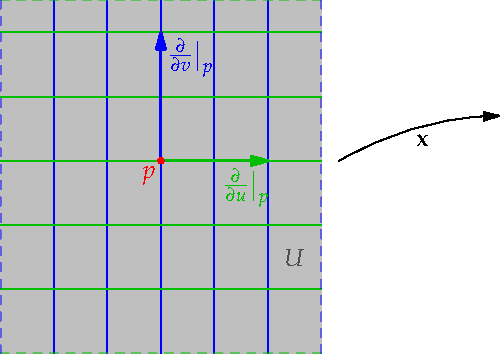
\includegraphics[scale=0.95]{surfaces-paramU}\quad	\href{http://www.math.uci.edu/~ndonalds/math162a/surfaces-param.html}{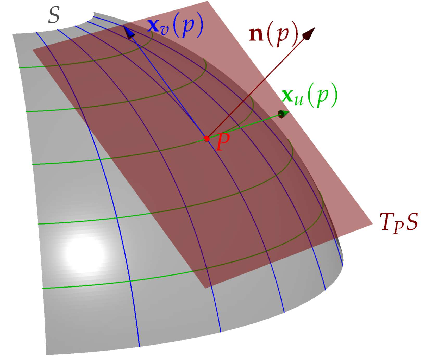
\includegraphics[scale=0.95]{surfaces-param}}
\end{center}


The partial derivatives $\vx_u(p),\vx_v(p)$ are \emph{tangent to the surface} at $\vx(p)$: if $p=(u_0,v_0)$ then the \emph{curve} $\vy(t):=\vx(t,v_0)$ lies in the surface and passes through $P=\vx(p)$; its tangent vector at $P$ is then
\[
	\vy'(u_0)=\lim_{h\to 0}\frac{\vy(u_0+h)-\vy(u_0)}h =\lim_{h\to 0}\frac{\vx(u_0+h,v_0)-\vx(p)}h  =\vx_u(p)
\]

\goodbreak
 

To help distinguish between domain and codomain, we standardize notation.
\begin{description}
	\item[\normalfont\emph{Domain} $U\subseteq\R^2$:]
	\begin{description}\itemsep2pt
		\item[\normalfont\emph{Points}\!]are written \emph{lower case} or as \emph{row vectors}: e.g.,\ $p=(u_0,v_0)\in U$. Typically we'll use $u,v$ as \emph{co-ordinates} unless it is more natural to use angles such as $\phi,\theta$.
		\item[\normalfont\emph{Tangent vectors/fields}\!]are written with an arrow in our \emph{new} notation: e.g.,\ $\vec w_p=\partialsat up\in T_p\R^2$.
	\end{description} 
	
	\item[\normalfont\emph{Codomain} $\E^3$:]
	\begin{description}\itemsep2pt
		\item[\normalfont\emph{Points}\!]are written \emph{upper case} or as \emph{row vectors,} e.g.,\ $P=(3,4,8)\in\E^3$. Co-ordinates on $\E^3$ will typically be $x,y,z$.
		\item[\normalfont\emph{Vectors}\!]are written \emph{bold-face} as either row or column vectors: e.g.,\ $\vx(u,v)=\bigl(u,v,u^2+v^2\bigr)$.
		\item[\normalfont\emph{Tangent vectors/fields}\!]use the \emph{old} notation:\footnotemark{} e.g.,\ if $P=\vx(p)$, then $\vx_u(p)=\partialsat[\vx]{u}p\in T_P\E^3$.
	\end{description} 
\end{description}

\footnotetext{
	To use our new notation in $\E^3$ would require a subtle redefinition of $\dvx$: if $\vec w$ is a vector field on $U$, then $\dvx(\vec w)$ is the vector field on $S$ such that $\bigl(\dvx(\vec w)\bigr)[f]=\vec w\bigl[f\circ\vx\bigr]$ for all $f:S\to\R$. In co-ordinates this benefits from  tensor notation:
	\[
		\vx(u_1,u_2)=\Bigl(x_1(u_1,u_2),x_2(u_1,u_2),x_3(u_1,u_2)\Bigr)\implies \dvx=\sum_{i,j}\partials[x_j]{u_i}\partials{x_j}\otimes\du_i
	\]
	In more general situations this approach is necessary, but it is overkill for our purposes!
}

\begin{example}{}{spherepolar}
	Consider the sphere of radius $a$ parametrized using spherical polar co-ordinates:
	\[
		\vx(\theta,\phi) 
			=a\!\threevec{\cos\theta\cos\phi}{\sin\theta\cos\phi}{\sin\phi}\!,\quad \dvx =\vx_\theta\,\dth+\vx_\phi\,\D\phi 
			=a\cos\phi\threevec{-\sin\theta}{\cos\theta}{0}\!\dth +a\!\threevec{-\cos\theta\sin\phi}{-\sin\theta\sin\phi}{\cos\phi}\!\D\phi
	\]
	The unit normal field is simply $\vn=\frac 1a\vx$. The domain $U=(0,2\pi)\times(-\frac\pi 2,\frac\pi 2)$ is an open rectangle whose image $S=\vx(U)$ is the sphere minus the (dashed) semicircle $\vx(0,\phi)$. While we could extend $\theta$ to wrap round the equator, we cannot extend to the north or south poles without sacrificing \emph{regularity}:
	\[
		\vx_\theta=a\cos\phi\threevec{-\sin\theta}{\cos\theta}{0}=\V0\text{ when }\phi=\pm\frac\pi 2
	\]
	\begin{minipage}{0.55\linewidth}\vspace{5pt}
		\hfill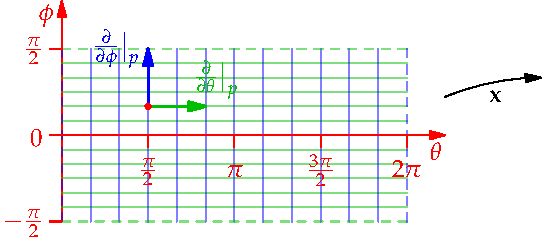
\includegraphics[scale=0.95]{surfaces-sphere2}
	\end{minipage}
	\hfill
	\begin{minipage}{0.44\linewidth}\vspace{-55pt}
		\flushright	\href{http://www.math.uci.edu/~ndonalds/math162a/surfaces-sphere.html}{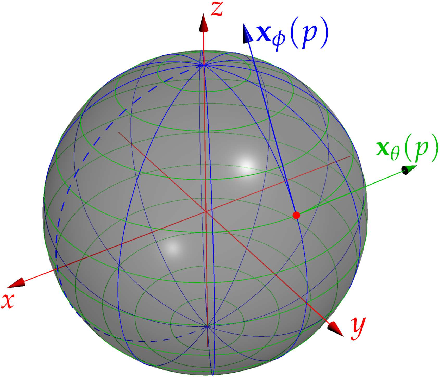
\includegraphics[scale=0.9]{surfaces-sphere}}
	\end{minipage}
	\medbreak
 	This illustrates the term \emph{local}: indeed the famous \emph{hairy ball theorem} from topology says that it is impossible to find a regular parametrization of the entire sphere by a single function.
 	\par
	Also observe how the tangent vectors $\smash[b]{\partialsat\phi p,\partialsat\theta p}\in T_p\R^2$ are mapped by $\dvx$ to tangent vectors
	\[
		\diffat[\vx]{\phi}p=\dvx\left(\partialsat\phi p\right),\quad \diffat[\vx]{\theta}p=\dvx\left(\partialsat\theta p\right)\in T_{\vx(p)}S
	\]
\end{example}

\goodbreak

\begin{thm}{}{}
	Let $S=\vx(U)$ be a smooth surface containing the point $P=\vx(p)$:
	\begin{enumerate}
	  \item The differential at $p$ is a linear map $\dvx:T_p\R^2\to T_P\E^3$ mapping tangent vectors in $\R^2$ to vectors tangent to $S$.
	  \item $S$ is regular at $P$ if and only if $\dvx$ is \emph{injective (1--1)} at $p$. In such a case we can view it as an invertible linear map $\dvx:T_p\R^2\to T_PS$.
	\end{enumerate}
\end{thm}

\begin{proof}
	\begin{enumerate}
	  \item The differential at $p$ is linear since the co-ordinate 1-forms $\du,\dv$ are linear: indeed
	  \begin{align*}
	  \dvx\left(a\partialsat up+b\partialsat vp\right)&=\vx_u(p)\,\du\left(a\partialsat up+b\partialsat vp\right)+\vx_v(p)\,\dv\left(a\partialsat up+b\partialsat vp\right)\\
	  &=a\vx_u(p)+b\vx_v(p) =a\,\dvx\left(\partialsat up\right)+b\,\dvx\left(\partialsat vp\right)
	  \end{align*}
	  This expression is moreover tangent to $S$ at $\vx(p)$: if this last assertion is unconvincing, see Exercise \ref{exs:tangentsurface}.

		\item The range of $\dvx$ at $p$ is plainly $\Span\{\vx_u(p),\vx_v(p)\}$. This is 2-dimensional (and thus defines the tangent plane) if and only if $\Rank \dvx=2\iff \dvx$ is 1--1.\qedhere
	\end{enumerate}
\end{proof}

It is worth reiterating two crucially important properties of $\dvx$:
\begin{itemize}
  \item At a regular point, $\dvx:T_p\R^2\to T_PS$ is an \textcolor{red}{invertible linear map}. We shall shortly use this to \emph{pull-back} calculations from $S$ to $U$.
  \item The differential is \textcolor{red}{co-ordinate independent} and thus does not depend on the parametrization of $S$. This follows since $\dvx$ is the unique 1-form satisfying $\dvx(\vec w)=\vec w[\vx]$ for all vector fields $\vec w$ on $U$; a description that does not depend on co-ordinates.
\end{itemize}


\begin{aside}\phantomsection\label{aside:coc}
	\boldinline{Aside: change of co-ordinates}\quad To more clearly spell this out, suppose we choose a new parametrization $\vy(s,t)=\vx\bigl(F(s,t)\bigr)$ where $F(s,t)=(u,v)$ is a change of co-ordinates on $U$. By the chain rule,
	\[
		\twovec{\vy_s}{\vy_t}=
		\begin{pmatrix}
			\partials[u]{s}&\partials[v]{s}\\
			\partials[u]{t}&\partials[v]{t}
		\end{pmatrix}
		\twovec{\vx_u}{\vx_v} \quad\text{and}\quad
		(\du\ \dv)=(\ds\ \dt)
		\begin{pmatrix}
			\partials[u]{s}&\partials[v]{s}\\
			\partials[u]{t}&\partials[v]{t}
		\end{pmatrix}
	\]
	from which
	\begin{align*}
		\D\vy&=(\ds\ \dt)\twovec{\vy_s}{\vy_t} =(\du\ \dv)
		\begin{pmatrix}
			\partials[u]{s}&\partials[v]{s}\\
			\partials[u]{t}&\partials[v]{t}
		\end{pmatrix}^{-1}
		\begin{pmatrix}
			\partials[u]{s}&\partials[v]{s}\\
			\partials[u]{t}&\partials[v]{t}
		\end{pmatrix}
		\twovec{\vx_u}{\vx_v} =(\du\ \dv)\twovec{\vx_u}{\vx_v}=\dvx
	\end{align*}
	The matrix of partial derivatives is the \emph{Jacobian} of the co-ordinate change.
	\smallbreak
	To be completely strict, $\dvx$ and $\D\vy$ are not identical since they feed on tangent vectors with respect to different co-ordinates. Formally
	\[
		\vy=\vx\circ F\implies\D\vy=\dvx\circ\D F
	\]
	where $\D F$ maps tangent vectors in $\Span\{\partials s,\partials t\}$ to those in $\Span\{\partials u,\partials v\}$: in matrix language, $\D F$ is precisely the above Jacobian!
\end{aside}


\boldsubsubsection{Common Surfaces}

You should have met many of these families/examples in multi-variable calculus.

\boldinline{Graphs} If $f(x,y)$ is a smooth function, its graph may be parametrized by $\vx(u,v)=\bigl(u,v,f(u,v)\bigr)$. Its differential and unit normal field are
	\[
		\dvx=\threevec 10{f_u}\du+\threevec 01{f_v}\dv\qquad \vn=\frac 1{\sqrt{1+f_u^2+f_v^2}}\threevec{-f_u}{-f_v}1
	\]
	This is regular at all points, regardless of $f$.


\begin{examples}{}{}
	\exstart The standard circular paraboloid may be parametrized $\vx(u,v)=\bigl(u,v,u^2+v^2\bigr)$.
	\begin{enumerate}\setcounter{enumi}{1}
	  \item The upper half of the unit sphere is the graph of $z=f(x,y)=\sqrt{1-x^2-y^2}$ where $x^2+y^2<1$.
	  
	  \item A plane has equation $ax+by+cz=d$ where $a,b,c,d$ are constant. Since at least one of $a,b,c$ must be non-zero, this may be written as a function and graphed. For instance, if $b\neq 0$ we have $y=f(x,z)=\frac 1b(d-ax-cz)$ and $\vn=\frac 1{\sqrt{a^2+b^2+c^2}}\bigl(a,b,c\bigr)$.
	\end{enumerate}
\end{examples}


\boldinline{Surfaces of Revolution} If a smooth positive function $x=f(z)$ is rotated around the $z$-axis, we obtain a parametrization
	\[
		\vx(\theta,v)=\bigl(f(v)\cos\theta,f(v)\sin\theta,v\bigr),\quad (\theta,v)\in(0,2\pi)\times\dom(f)
	\]
	with differential and unit normal field
	\begin{gather*}
		\dvx =\threevec{-f(v)\sin\theta}{f(v)\cos\theta}0\dth+\threevec{f'(v)\cos\theta}{f'(v)\sin\theta}1\dv\qquad \vn =\frac 1{\sqrt{1+f'(v)^2}}\threevec{\cos\theta}{\sin\theta}{-f'(v)}
	\end{gather*}


\begin{examples}{}{}
	\exstart The simplest example ($f(z)\equiv 1$) is the right circular cylinder of radius 1.
	\begin{enumerate}\setcounter{enumi}{1}
	  \begin{minipage}[t]{0.56\linewidth}\vspace{0pt}
	  \item We may rotate around any axis! For instance, if we rotate the curve $z=2+\cos x$  around the $x$-axis, the resulting surface may be parametrized
	  \[
	  	\vx(\theta,v)=(2+\cos v)\!\threevec{0}{\cos\theta}{\sin\theta}+\threevec v00
		\]
		This time $v$ measures distance along the $x$-axis and $\theta$ the angle of rotation around it.
		\smallbreak
		The differential and unit normal field are
	  \end{minipage}
	  \hfill
	  \begin{minipage}[t]{0.39\linewidth}\vspace{-10pt}
			\flushright	\href{http://www.math.uci.edu/~ndonalds/math162a/surfaces-revol.html}{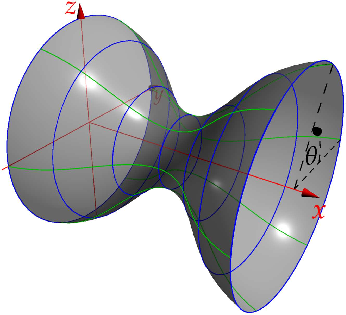
\includegraphics{surfaces-revol}}
	  \end{minipage}
	  \par%\vspace{-10pt}
	  \begin{gather*}
	  	\dvx=(2+\cos v)\!\threevec 0{\!-\sin\theta\!}{\cos\theta}\!\dth+\threevec{1}{\!-\sin v\cos\theta\!}{\!-\sin v\sin\theta\!}\!\dv \qquad
	  	\vn=\frac 1{\sqrt{1+\sin^2\!v}}\threevec{\sin v}{\cos\theta}{\sin\theta}
	  \end{gather*}
	  Note the \emph{orientation} of the surface: the unit normal field points \emph{outward,} away from the $x$-axis.
	\end{enumerate}
\end{examples}


\goodbreak


\boldinline{Ruled Surfaces} Given functions $\vy(u),\vz(u)$, define
	\[
		\vx(u,v)=\vy(u)+v\vz(u)
	\]
	Through each point $P=\vx(u_0,v_0)$ passes a line $t\mapsto \vx(u_0,t)=\vy(u_0)+t\vx(u_0)$ lying in the surface. The surface can be visualized as moving a \emph{ruler} through space. Ruled surfaces are common in engineering applications since they may be constructed using straight beams.
	
\begin{defn}{}{}
	The \emph{tangent developable} of a smooth curve $\vy$ is the special case when $\vz=\vy'$.
\end{defn}

\begin{examples}{}{}
	\exstart Every plane is a ruled surface! Let $\vy$ be a line in the plane and $\vz$ any other tangent direction. For instance, the plane passing through $(1,0,9)$ and spanned by $(2,-3,-5)$ ad $(1,2,3)$ may be parametrized
	\[
		\vx(u,v)%=\underbrace{\threevec{1+2u}{-3u}{9-5u}}_{\vy(u)}+v\underbrace{\threevec 123}_{\vz(u)}
		=\underbrace{\bigl(1,0,9\bigr)+\bigl(2,-3,-5\bigr)u}_{\vy(u)}+\underbrace{\bigl(1,2,3\bigr)}_{\vz(u)}\!v
	\]
	\begin{enumerate}\setcounter{enumi}{1}
		\item A \emph{helicoid} is built by joining each point of a helix to its axis of rotation. From the standard helix, we obtain the helicoid $\vx(u,v)=\bigl(v\cos u,v\sin u,u\bigr)$ for $v>0$.
	  \item\label{page:hyperrule} The \emph{hyperboloid of one sheet} is a \emph{doubly ruled surface}: through each point there are \emph{two} lines lying on the surface. It may be parametrized as a ruled surface by
		\[
			\vx(u,v)=\threevec 100+u\threevec 011+v\threevec{2u}{u^2-1}{u^2+1}
		\]
	though convincing yourself there are \emph{two} lines through each point takes a little more work\ldots
	
		\begin{center}
			\begin{tabular}{c@{\qquad\qquad}c}
				\href{http://www.math.uci.edu/~ndonalds/math162a/surfaces-helicoid.html}{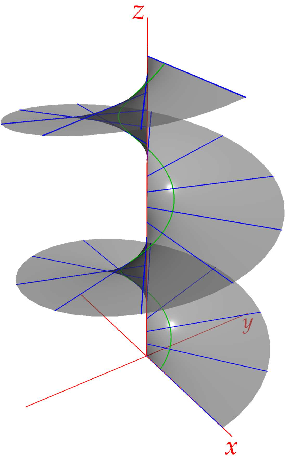
\includegraphics{surfaces-helicoid}}
				&
				\href{http://www.math.uci.edu/~ndonalds/math162a/surfaces-hyper.html}{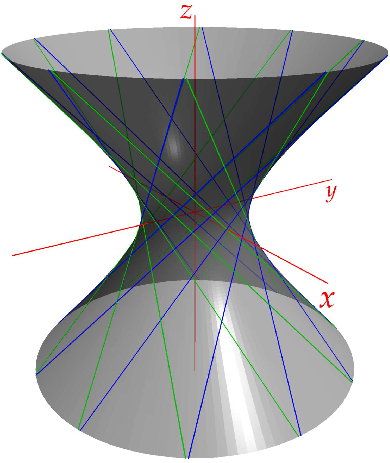
\includegraphics{surfaces-hyper}}
				\\
				Helicoid
				&
				Hyperboloid
			\end{tabular}
		\end{center}
	
	\end{enumerate}
\end{examples}



\boldsubsubsection{Implicitly Defined Surfaces}


\begin{defn}{}{}
	A \emph{regular implicitly defined surface} is the zero set of a smooth function $f:\E^3\to\R$ for which $\df\neq 0$ (equivalently $\nabla f\neq \V0$).
\end{defn}

Recall that the directional derivative of $f$ in the direction $\vv$ is $D_{\vv}f(P)=\vv\cdot\nabla f(P)$. This is zero if and only if $\vv$ is orthogonal to $\nabla f(P)$. In particular, this says that $\nabla f$ provides a \emph{normal field} to an implicitly defined surface.

\begin{examples}{}{}
	\exstart Let $a,b,c,d$ be constants. The function $f(x,y,z)=ax+by+cz-d$ has 
	\[
		\df=a\,\dx+b\,\dy+c\,\dz
	\]
	which is non-zero provided at least one of $a,b,c$ are non-zero. This defines a plane with unit normal field $\vn=\frac 1{\Nm{\nabla f}}\nabla f=\frac 1{\sqrt{a^2+b^2+c^2}}\bigl(a,b,c\bigr)$.
	\begin{enumerate}\setcounter{enumi}{1}
	  \item The sphere of radius $a$ is the zero set of $f(x,y,z)=x^2+y^2+z^2-a^2$. It has unit normal field
	  \[
	  	\vn=\frac 1{\Nm{\nabla f}}\nabla f=\frac 1a\bigl(x,y,z\bigr)
	  \]
	The sphere is everywhere regular since at least one of $x,y,z$ is non-zero at all points of the sphere. Contrast this with our earlier example of the \emph{parametrized} sphere which could not be made regular at the north and south poles. The lack of regularity in this case is an aspect of the parametrization, not the surface itself.
		\item The function $f(x,y,z)=x^2+y^2-z^2-c$ has
		\[
			\df=2(x\,\dx+y\,\dy-z\,\dz)
		\]
		which is non-zero away from $(x,y,z)=(0,0,0)$. Depending on the sign of $c$, the zero set is a hyperboloid or a cone; visualize the horizontal cross-sectional circles to determine which.
		\begin{quote}
	  	$c>0$\quad \textcolor{Turquoise}{Hyperboloid of 1-sheet}: $x^2+y^2=z^2+c>0$ for all $z$\smallbreak
	  	$c=0$\quad \textcolor{Magenta}{Cone}: $x^2+y^2=z^2$ contains a non-regular point $(0,0,0)$\smallbreak
	  	$c<0$\quad \textcolor{Goldenrod}{Hyperboloid of 2-sheets}: $x^2+y^2=z^2-\nm c\ge 0$ only when $\nm z\ge \sqrt{\nm c}$
		\end{quote}
		\begin{center}
			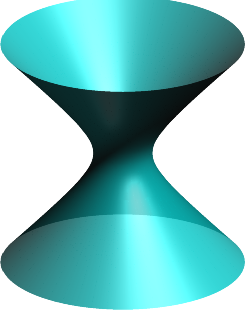
\includegraphics{surfaces-hyper1} \qquad 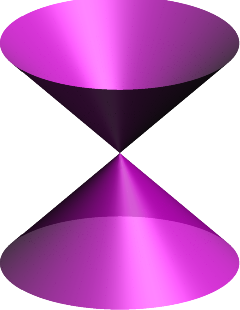
\includegraphics{surfaces-cone} \qquad 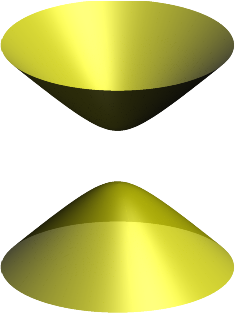
\includegraphics{surfaces-hyper2}
		\end{center}
	\end{enumerate}
\end{examples}

Our next result, a corollary of the famous \emph{implicit function theorem,} ties together the notions of \emph{regularity.} In particular, it says that we can always assume the existence of \emph{local} co-ordinates.

\begin{thm}{}{implicit}
	A regular implicitly defined surface $f(x,y,z)=0$ is (locally) the image of a regular local surface.
\end{thm}

\begin{proof}
	Suppose $P=(x_0,y_0,z_0)$ lies on the surface and $\nabla f(P)\neq\V0$. At least one of the partial derivatives of $f$ is non-zero; suppose WLOG that $f_z(P)\neq 0$. By the implicit function theorem, there exists $U\subseteq\R^2$ and a function $g:U\to\R$ for which $g(x_0,y_0)=z_0$ and $f\big(x,y,g(x,y)\big)=0$. The surface is then (locally) the graph of $z=g(x,y)$.
	\[
		\vx:U\to\E^3:(u,v)\mapsto\bigl(u,v,g(u,v)\bigr) \tag*{\qedhere}
	\]
\end{proof}


\begin{example}{}{hyperboloid1sheet}
	The zero set of $f(x,y,z)=x^2+y^2-z^2-6$ is a hyperboloid of one sheet. It has unit normal vector field
	\[
		\vn(x,y,z)=\frac 1{\Nm{\nabla f}}\nabla f=\frac{1}{\sqrt{x^2+y^2+z^2}}\threevec{x}{y}{-z} =\frac{1}{\sqrt{6+2z^2}}\threevec{x}{y}{-z}
	\]
	whenever $(x,y,z)$ is a point on the hyperboloid. For instance, at $P=(3,1,2)$ the unit normal is $\vn(P)=\frac{1}{\sqrt{14}}(3,1,2)$ and the tangent plane has equation
	\[
		3x+y-2z=6
	\]
	Alternatively, the hyperboloid can be parametrized in several ways.
	\begin{enumeratea}
		\item In the language of the proof, near $P=(3,1,2)$ it is the graph of $z=g(x,y)=\sqrt{x^2+y^2-6}$. This results in a (local) regular parametrization
		\[
			\vx(u,v)=\bigl(u,v,\sqrt{u^2+v^2-6}\bigr)
		\]
		\item The hyperboloid is a surface of revolution around the $z$-axis:
		\[
			\vx(\theta,v) =\threevec{\sqrt{6+v^2}\cos\theta}{\sqrt{6+v^2}\sin\theta}v
		\]
		For this parametrization, the differential and normal field are
		\begin{gather*}
			\dvx=\sqrt{6+v^2}\threevec{-\sin\theta}{\cos\theta}0\!\dth +\frac 1{\sqrt{6+v^2}}\threevec{v\cos\theta}{v\sin\theta}{\sqrt{6+v^2}}\dv\\
			\vn=\frac{\vx_\theta\times\vx_v}{\Nm{\vx_\theta\times\vx_v}} =\frac 1{\sqrt{6+2v^2}} \threevec{\sqrt{6+v^2}\cos\theta}{\sqrt{6+v^2}\sin\theta}{-v}
		\end{gather*}
	 	which is precisely what we obtained above.
	\end{enumeratea}
	Yet another expression could be obtained using a parametrization as a ruled surface (e.g.,\ page \pageref{page:hyperrule}).
\end{example}



\begin{exercises}
	\exstart Show that parametrization $\vx(r,\theta)=\bigl(r\cos\theta,r\sin\theta,\sqrt{1-r^2}\bigr)$ of the upper hemisphere is non-regular at $r=0$.

	\begin{enumerate}\setcounter{enumi}{1}
	  \item Explain why the parametrization in Example \ref{ex:hyperboloid1sheet}(a) is \emph{local}: what is left out?
	  
	  \item\label{exs:paraboloid}
	  \begin{enumerate}\itemsep0pt
	    \item Compute $\dvx$ and $\vn$ for the paraboloid $\vx(u,v)=\bigl(u,v,u^2+v^2\bigr)$.
	  	\item Repeat for the polar co-ordinate parametrization $\vy(r,\theta)=\bigl(r\cos\theta,r\sin\theta,r^2\bigr)$. Is this parametrization everywhere regular?
			\item Using $x=r\cos\theta$, etc., write $\dvx$ in terms of $r,\theta,\dr,\dth$. What do you observe?
			\item By viewing the paraboloid as the zero set of $f(x,y,z)=z-x^2-y^2$, find another expression for the unit normal field.
		\end{enumerate}
	
	  \begin{minipage}[t]{0.77\linewidth}\vspace{-2pt}
			\item\label{exs:tandev}
			\begin{enumerate}\itemsep0pt
			  \item Find a parametrization for the tangent developable of the helix $\vy(u)=\bigl(\cos u,\sin u,u\bigr)$. Compute $\D\vy$ and the unit normal field $\vn$.\par
	    (\emph{The picture covers $v\in(-3,6)$ with the original curve $\vy(u)$ in \textcolor{Green}{green}})
	    	\item If $\vy$ is a unit speed biregular curve, prove that its tangent developable $\vx(u,v)=\vy(u)+v\vy'(u)$ is a regular surface except when $v=0$. Express the differential and unit normal field in terms of the Frenet frame of $\vy$.
	    \end{enumerate}
	  
	  	\smallskip
	    	
	  	\item Let $f(x,y,z)=z^2$. Show that the zero set of $f$ has a regular parametrization despite  the gradient of $f$ vanishing at $z=0$.
	  \end{minipage}
	  \hfill
	  \begin{minipage}[t]{0.21\linewidth}\vspace{-14pt}  			\flushright	\href{http://www.math.uci.edu/~ndonalds/math162a/surfaces-tandev.html}{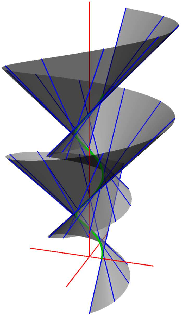
\includegraphics{surfaces-tandev}}
	  \end{minipage}
	  
	
		\item Let $a,b,c$ be positive constants and define $\vx(\theta,\phi)=\smash{\sthreevec{a\cos\theta\cos\phi}{b\sin\theta\cos\phi}{c\sin\phi}}$, $(\theta,\phi)\in(0,2\pi)\times(-\frac\pi 2,\frac\pi 2)$
		\begin{enumerate}\itemsep0pt
			\item Show that $\vx$ parametrizes the ellipsoid $\frac{x^2}{a^2}+\frac{y^2}{b^2}+\frac{z^2}{c^2}=1$.	What part(s) of the ellipsoid are `missing' from the parametrization?
			\item Describe geometrically the curves $\theta=\,\,$constant and $\phi=\,\,$constant on the ellipsoid.
			\item Calculate the differential of $\vx$ and show that $\dvx$ is 1--1 for each $p\in U$.
			%\item Find the normal vector field of the ellipsoid in terms of $x,y,z$.
		\end{enumerate}
		
		
		\begin{minipage}[t]{0.75\linewidth}\vspace{-8pt}
			\item The tube of radius $a>0$ centered on a curve $\vy(t)$ may be parametrized in terms of the Frenet frame of $\vy$:
			\[
				\vx(\phi,t)=\vy(t)+a\cos\phi\,\vN(t)+a\sin\phi\,\vB(t)
			\]
			\begin{enumerate}
			  \item \emph{Briefly} explain why the normal field is $\vn=\cos\phi\,\vN(t)+\sin\phi\,\vB(t)$.
			  \item Suppose $\vy$ is unit speed. Prove that $\vx$ is everywhere regular if and only if $\kappa(t)<\frac 1a$ at all points of the generating curve.
			\end{enumerate}
		  
			\item\label{exs:tangentsurface} Let $c(t):(-\epsilon,\epsilon)\to U$ be a curve and $\vy(t)=\vx\bigl(c(t)\bigr)$ the corresponding curve in the surface $\vx:U\to\E^3$. Prove that $\dvx\bigl(c'(0)\bigr)=\vy'(0)$.\par
			(\emph{Hint: Recall how to write $c'(t)$ as a \emph{vector field}}) 
			
				
			\item\label{exs:mobius} (Möbius strip)\lstsp Show that $\vx(u,v)=\sthreevec{(2+v\cos\frac u2)\cos u}{(2+v\cos\frac u2)\sin u}{v\sin\frac u2}$ is regular and orientable whenever $0<u<2\pi$ and $-1<v<1$. By computing $\vn(0,0)$ and $\vn(2\pi,0)$, explain what happens if we try to extend $u$ to $[0,2\pi]$.
	  \end{minipage}
	  \hfill
	  \begin{minipage}[t]{0.23\linewidth}\vspace{-15pt}
	  	\flushright
			\href{http://www.math.uci.edu/~ndonalds/math162a/surfaces-helixtube.html}{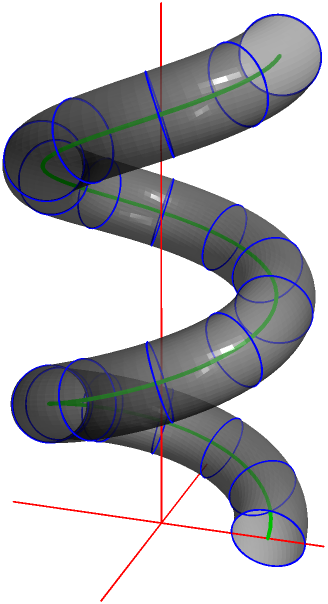
\includegraphics{surfaces-helixtube}}\\
			\href{http://www.math.uci.edu/~ndonalds/math162a/surfaces-mobius.html}{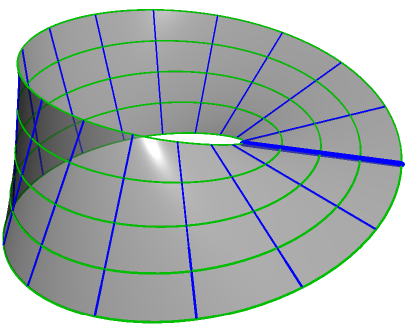
\includegraphics{surfaces-mobius}}
	  \end{minipage}
	  


	
	
	% 	\item Let $r>a>0$ be constants. The zero set of the function $f(x,y,z)=(\sqrt{x^2+y^2}-r)^2+z^2-a^2$ defines a \emph{torus}.
	% 	\begin{enumerate}
	%   	\item Find a unit normal field for the torus.
	%   	\item Let $z=a\sin\phi$. Why can we choose $\phi$ to be a co-ordinate on the torus? Find a parametrization $\vx(\phi,\theta)$ of the torus where $\phi$ is one of the co-ordinates. Compute the tangent vectors $\vx_\phi$ and $\vx_\theta$ and check that $\vx_\phi\times\vx_\theta$ is a normal vector field.
	%   	%\item Explain why topologists often talk about the torus as a square whose opposite edges have been glued together. How does this relate to parameterizing the torus?
	%   	\item Show that the zero set of $f$ does not define a regular surface when $a=0$ or when $r=a$. What has happened to the torus in each case?
	% 	\end{enumerate}
	  
	
	  

		
		
	
	
	% 
	%     \item* Suppose that $A:U\to M_{n\times n}$ is a differentiable function into the set of $n\times n$ matrices ($M_{n\times n}=\R^{n^2}$ so we know what differentiable means). Suppose also that $A(p)$ is invertible for every $p\in U$. We can think about the matrix-valued 1-form $\D A$ on $U$.
	%   \begin{enumerate}
	%     \item By differentiating $A^{-1}A=\mathrm I$ (use the product rule!), find the differential $\D(A^{-1})$ in terms of $\D A$.
	%     \item Suppose that every matrix $A(p)$ is orthogonal ($A^{-1}(p)=A^T(p)$) and define the matrix-valued 1-form $W=A^{-1}\D A$. Prove, using part (a), that $W^T=-W$.%\\
	%     %(\emph{An example is where $A=(\ve_1,\ldots,\ve_n)$ is a frame, and $W$ is the matrix of $w_{ij}$ in the structure equations})
	%   \end{enumerate}
		
		
	\end{enumerate}
\end{exercises}


\clearpage

\subsection{The Fundamental Forms}\label{sec:fund}

Our immediate goal is to use differentials to describe the shape of a surface. Before making the main definition, we need  another product of 1-forms.

\begin{defn}{}{}
	Given 1-forms $\alpha,\beta$ on $U$, define the \emph{symmetric 2-form} $\alpha\beta$ by
	\[
		\alpha\beta(\vec v,\vec w) =\frac{1}{2}\bigl(\alpha(\vec v)\beta(\vec w)+\alpha(\vec w)\beta(\vec v)\bigr)
		\]
	where $\vec v,\vec w$ are vector fields on $U$. Note that $\alpha^2(\vec v,\vec w):=\alpha\alpha(\vec v,\vec w)=\alpha(\vec v)\alpha(\vec w)$.
\end{defn}

Symmetric 2-forms behave the way you (hopefully!) think they should.

\begin{lemm}{}{}
	On each tangent space, $\alpha\beta:T_p\R^n\times T_p\R^n\to\R$ is a symmetric and bilinear.\par
	Moreover $\alpha\beta=\beta\alpha$, and the product is linear in each slot:
	\[
		\alpha(\beta+\gamma)=\alpha\beta+\alpha\gamma\quad\text{and}\quad (\alpha+\beta)\gamma=\alpha\gamma+\beta\gamma
		\tag{$\ast$}
	\]
\end{lemm}

% \begin{proof}
% Symmetry: $\alpha\beta(v,w)=\alpha\beta(w,v)$ is clear from the formula.\smallbreak
% Linearity in 1\st\ slot: if we fix $w_p\in T_p\R^n$, we see that $\alpha\beta(-,w_p):v_p\to \alpha\beta(v_p,w_p)$ is linear since both 1-forms are are linear. By symmetry we have bilinearity.
% \end{proof}

Take care when using co-ordinate 1-forms; convention dictates that $\dx^2=(\dx)^2$ is a symmetric 2-form, \emph{not} the exterior derivative (1-form) $\D(x^2)=2x\,\dx$.

\begin{example}{}{}
	Let $\vec v=a\partials x+b\partials y$ and $\vec w=c\partials x+d\partials y$. Then
	\[
		\dx^2(\vec v,\vec w)=ac,\qquad \dy^2(\vec v,\vec w)=bd,\qquad \dx\,\dy(\vec v,\vec w)=\frac 12(ad+bc)
	\]
	In particular, $\bigl(\dx^2+\dy^2\bigr)(\vec v,\vec w)=ac+bd$ is the \emph{dot product} in disguise.\smallbreak
	To evaluate symmetric 2-forms with respect to co-ordinates, linearity and distributivity ($\ast$) are all you need. For instance, if $\alpha =x\,\dx-\dy$ and $\beta =xy\,\dy$, then $\alpha\beta=x^2y\,\dx\dy-xy\,\dy^2$.
\end{example}


If $\alpha,\beta$ take values in $\E^n$, we use the dot product for multiplication of the resulting \emph{vectors} $\alpha(\vec v)$, etc.
\[
	(\alpha\cdot\beta)(\vec v,\vec w):=\frac 12\bigl(\alpha(\vec v)\cdot\beta(\vec w)+\alpha(\vec w)\cdot\beta(\vec v)\bigr)
\]

\begin{defn}{}{fund}
	The \emph{first and second fundamental forms} of a regular local surface $\vx:U\to\E^3$ are
	\[
		\I=\dvx\cdot\dvx,\qquad \II=-\dvx\cdot\dvn
	\]
	where $\dvn$ is the differential of the unit normal field ($\II$ requires that the surface be \emph{oriented}). The first fundamental form is also commonly denoted $\ds^2$ (see Example \ref{ex:spherepolar2} and Theorem \ref{thm:fundformcurves} for why).
\end{defn}


\begin{example}{}{}
	If $\vx(u,v)=\bigl(u,uv,1+u\bigr)$, then 
	\[
		\dvx=\threevec 1v1\du+\threevec 0u0\dv,\qquad \vn=\frac 1{\sqrt 2}\threevec 10{-1},\qquad \dvn=\V0
	\]
	from which $\I=(2+v^2)\,\du^2+2uv\,\du\,\dv+u^2\,\dv^2$ and $\II=0$.
\end{example}

\goodbreak


\boldinline{Why should we care about $\I$ \& $\II$?}

\begin{description}
	\item[\normalfont\emph{Basic interpretation}]\phantomsection\label{sec:formsmeaning} $\I(\vec v,\vec w)=\dvx(\vec v)\cdot\dvx(\vec w)$ pulls back the dot product from $T_PS$ to $T_p\R^2$. The length of and angle between tangent vectors to the surface $S$ at $P$ may now be computed in $T_p\R^2$.\par
	 	$\II(\vec v,\vec w)=-\frac 12\bigl(\dvx(\vec v)\cdot\dvn(\vec w)+\dvx(\vec w)\cdot\dvn(\vec v)\bigr)$ describes how the normal field $\vn$ changes over the surface. In the example, $\II\equiv 0$ encapsulates the \emph{constancy} of the normal field: the surface is (part of) the plane $\vx\cdot(1,0,-1)=-1$.
	
	\item[\normalfont\emph{Co-ordinate invariance}] Since $\dvx$ is independent of co-ordinates, so also is $\I$. The unit normal field is independent of \emph{oriented} co-ordinate changes. More formally, if $\vy(s,t)=\vx(u,v)$ parametrize the same surface, then\footnote{As in the Aside on page \pageref{aside:coc}, we strictly have $\I_\vy=\I_\vx\circ \D F$, etc., where $\vy(s,t)=\vx\bigl(F(s,t)\bigr)=\vx(u,v)$. The $\pm$-sign in the expressions for $\II$ is that of the \emph{determinant} of the Jacobian $\D F$.}
	\[
		\I_\vy=\I_\vx\quad \text{and}\quad \II_\vy=
		\begin{cases}
			\II_\vx&\text{if the orientations are identical}\\
			-\II_\vx&\text{if the orientations are reversed}
		\end{cases}
	\]
\end{description}

The upshot is that the fundamental forms provide a co-ordinate independent way to compute information about a surface from within the \emph{parametrization space} $U$.


\begin{example}{}{spherepolar2}
	For the sphere of radius $a$ in spherical polar co-ordinates, recall Example \ref{ex:spherepolar}:
	\begin{align*}
		\vx(\theta,\phi) =a\!\threevec{\cos\theta\cos\phi}{\sin\theta\cos\phi}{\sin\phi}&\implies\dvx =a\cos\phi\threevec{-\sin\theta}{\cos\theta}{0}\!\dth+a\!\threevec{-\cos\theta\sin\phi}{-\sin\theta\sin\phi}{\cos\phi}\!\D\phi\\[3pt]
		&\implies \I=a^2\bigl(\cos^2\!\phi\,\D\theta^2+\D\phi^2\bigr)
	\end{align*}
	If you revisit the pictures in Example \ref{ex:spherepolar}, the effect of $\I$ is easy to visualize:
	\begin{itemize}\itemsep2pt
	  \item $\I(\partials\theta,\partials\theta)=\Nm{\vx_\theta}^2=a^2\cos^2\!\phi$: the tangent vector $\vx_\theta$ is \emph{shorter} near the poles, where $\cos\phi\to 0$.
	  \item $\I(\partials\phi,\partials\phi)=\Nm{\vx_\phi}^2=a^2$: the tangent vector $\vx_\phi$ always has the \emph{same length.}
	  \item $\I(\partials\theta,\partials\phi)=\vx_\theta\cdot\vx_\phi=0$: the co-ordinate tangent vectors are always \emph{orthogonal.}
	\end{itemize}
	At a point $P=\vx(p)$ on the sphere, if we increase the co-ordinates by tiny quantities $\Delta p=\bigl(\Delta\theta,\Delta\phi)$, then the distance $\Delta s$ travelled along the surface approximately satisfies
	\[
		(\Delta s)^2\approx \Nm{\vx(p+\Delta p)-\vx(p)}\approx \Nm{\vx_\theta\,\Delta\theta+\vx_\phi\,\Delta\phi}^2= a^2\cos^2\!\phi\,(\Delta\theta)^2+a^2(\Delta\phi)^2
	\]
	with equality in the limit $\Delta\theta,\Delta\phi\to 0$. Near the poles, a change in \emph{longitude} $\Delta\theta$ corresponds to a smaller distance on the sphere. This is analogous to how a standard \emph{map} of the Earth works, with distances appearing distorted near the poles. We'll return to this idea shortly\ldots\smallbreak
	Computing $\II$ is very easy for the sphere, since $\vn=\frac 1a\vx$ is merely the scaled position vector:
	\[
		\II=-\dvx\cdot\dvn=-\frac{1}{a}\,\dvx\cdot\dvx=-\frac{1}{a}\I =-a\bigl(\cos^2\!\phi\,\D\theta^2+\D\phi^2\bigr)
	\]
\end{example}


\goodbreak

The fundamental forms $\I,\II$ may be computed directly in terms of co-ordinates $u,v$.
 
\begin{thm}{}{fundcoord}
	If $\vx:U\to\E^3$ is a regular (oriented) surface, then
	\[
		\I=E\,\du^2+2F\,\du\,\dv+G\,\dv^2\quad\text{and}\quad \II =l\,\du^2+2m\,\du\,\dv+n\,\dv^2
	\]
	where the smooth functions $E,F,G,l,m,n:U\to\R$ are defined by
	\begin{align*}
		&E=\vx_u\cdot\vx_u &&F=\vx_u\cdot\vx_v &&G=\vx_v\cdot\vx_v\\
		&l=\vx_{uu}\cdot\vn =-\vx_u\cdot\vn_u\quad &&m=\vx_{uv}\cdot\vn=-\vx_u\cdot\vn_v=-\vx_v\cdot\vn_u\quad &&n=\vx_{vv}\cdot \vn=-\vx_v\cdot\vn_v
	\end{align*}
\end{thm}

The expressions for $\II$ come from differentiating $\vx_u\cdot\vn=0=\vx_v\cdot\vn$, and are particularly helpful because they avoid computing derivatives of $\vn$ (which likely contains a square-root). 

\begin{example}{}{paraboloidpolar}
	Parametrize the graph of $z=f(x,y)$ by $\vx(u,v)=\bigl(u,v,f(u,v)\bigr)$ to obtain,
	\begin{gather*}
		\begin{aligned}
		\vx_u=\threevec 10{f_u}, \quad \vx_v=\threevec 01{f_v} &\implies E=1+f_u^2, \quad F=f_uf_v, \quad G=1+f_v^2\\
		&\implies \I=(1+f_u^2)\,\du^2+2f_uf_v\,\du\,\dv+(1+f_v^2)\,\dv^2
	\end{aligned}\\[8pt]
	\begin{aligned}
		\vx_{uu}=\threevec 00{f_{uu}}, \quad &\vx_{uv}=\threevec 00{f_{uv}}, \quad \vx_{vv}=\threevec 00{f_{vv}}, \quad \vn=\frac{1}{\sqrt{1+f_u^2+f_v^2}}\threevec{-f_u}{-f_v}{1}\\[2pt]
		\implies &l=\frac{f_{uu}}{\sqrt{1+f_u^2+f_v^2}}, \quad m=\frac{f_{uv}}{\sqrt{1+f_u^2+f_v^2}}, \quad n=\frac{f_{vv}}{\sqrt{1+f_u^2+f_v^2}}\\[2pt]
		\implies &\II=\frac{1}{\sqrt{1+f_u^2+f_v^2}} \left(f_{uu}\,\du^2 +2f_{uv}\,\du\,\dv+
		f_{vv}\,\dv^2\right)
	\end{aligned}
	\end{gather*}
	As a particular example, the circular paraboloid $z=x^2+y^2$ has fundamental forms
	\begin{gather*}
		\I=(1+4u^2)\,\du^2+8uv\,\du\,\dv+(1+4v^2)\,\dv^2 =\du^2+\dv^2+4\bigl(u\,\du+v\,\dv\bigr)^2\\[2pt]
		\II=\frac{2}{\sqrt{1+4u^2+4v^2}}\bigl(\du^2+\dv^2\bigr)
	\end{gather*}


	As a sanity check, compare with the parametrization of the same paraboloid in polar co-ordinates $\vy(r,\theta)=\bigl(r\cos\theta,r\sin\theta,r^2\big)$ (Exercise \ref*{sec:regularsurfaces}.\ref{exs:paraboloid}). By computing the partial derivatives $\vy_r,\vy_\theta,\vy_{rr},\vy_{r\theta},\vy_{\theta\theta}$ directly, one easily verifies that
	\begin{gather*}
	\I=(1+4r^2)\,\dr^2+r^2\,\dth^2,\qquad\II=\frac{2}{\sqrt{1+4r^2}}\big(\dr^2+r^2\,\dth^2\bigr)
	\end{gather*}
	These expressions are identical to the originals (same orientation!) since
	\[
		\begin{cases}
			\du=\cos\theta\,\dr-r\sin\theta\,\dth\\
			\dv=\sin\theta\,\dr+r\cos\theta\,\dth
		\end{cases}
		\implies
		\begin{cases}
			\du^2+\dv^2=\dr^2+r^2\,\dth^2\\
			\bigl(u\,\du+v\,\dv\bigr)^2=r^2\,\dr^2\\
		\end{cases} 
  \]
\end{example}

\goodbreak


\boldsubsubsection{Curves in Surfaces: interpreting $\I$ and $\II$}

Given a regular (oriented) surface $\vx:U\to\E^3$ and a curve $c(t)$ in $U$, we may transfer this curve to the surface $\vy(t)=\vx\bigl(c(t)\bigr)$. Its tangent vector (Exercise \ref*{sec:regularsurfaces}.\ref{exs:tangentsurface}) and speed are then
\[
	\vy'(t)=\dvx\bigl(c'(t)\bigr) \implies \Nm{\vy'(t)}=\sqrt{\dvx\bigl(c'(t)\bigr)\cdot\dvx\bigl(c'(t)\bigr)}=\sqrt{\I\bigl(c'(t),c'(t)\bigr)}
\]
We can do something similar for the second fundamental form.

\begin{thm}{}{fundformcurves}
Let $\vy(t)=\vx\bigl(c(t)\bigr)$ parametrize a curve in a surface $\vx$ with unit normal field $\vn$.
\begin{enumerate}
  \item If $a<b$, then the \emph{arc-length} of $\vy$ between $\vy(a)$ and $\vy(b)$ is $\smash{\int_a^b\sqrt{\I\bigl(c'(t),c'(t)\bigr)}\,\dt}$.
	\item The \emph{normal acceleration} of the curve is $\vy''(t)\cdot\vn=\II(c',c')$.
\end{enumerate}
\end{thm}

This puts some flesh on our earlier observations (page \pageref{sec:formsmeaning}). $\I$ measures \emph{infinitesimal squared-distance} on the surface, while $\II$ measures how the surface bends away from the normal field: recall how force/acceleration motivated the curvature $\kappa$ of a curve (Definition \ref{defn:curvature}).

\begin{proof}
\begin{enumerate}
  \item Arc-length is the integral of the speed $\Nm{\vy'(t)}=\smash{\sqrt{\I\bigl(c'(t),c'(t)\bigr)}}$.
  \item Since $\vy'$ lies in the tangent plane, we have $\vy'\cdot\vn\equiv 0$. Differentiate to obtain
  \begin{align*}
		0&=\diff t(\vy'\cdot \vn) =\vy''\cdot \vn+\vy'\cdot\diff t\vn\bigl(c(t)\bigr) =\vy''\cdot\vn+\dvx(c')\cdot\D\vn(c') =\vy''\cdot\vn-\II(c',c')\tag*{\qedhere}
	\end{align*}
\end{enumerate}
\end{proof}


%Skater example, then maps revisited, then hyp space?


\begin{example*}{\ref{ex:spherepolar2}, cont}{}%\phantomsection\label{ex:spherepolar3}
\hypertarget{ex:spherepolar4}
	Consider the \textcolor{blue}{curve} $c(t)=(\theta(t),\phi(t))=\bigl(2t,t\bigr)$ where $0\le t\le\frac\pi 4$. This has tangent field $c'(t)=2\partials\theta+\partials\phi$. Translated to the unit sphere, the resulting \textcolor{blue}{curve} has arc-length
	\[
		\int_0^{\frac\pi 4}\sqrt{\I\bigl(c',c')}\,\dt =\int_0^{\frac\pi 4}\sqrt{4\cos^2\!t+1}\,\dt \approx 1.619
	\]
	In the parametrization space $U$, \textcolor{blue}{$c(t)$} is a straight line. The shortest path between the endpoints of the curve \emph{on the sphere} is the \textcolor{Green}{great circle arc} with length $\frac{2\pi}4=\frac\pi 2\approx 1.571$; its \textcolor{Green}{pre-image} in $U$ \emph{appears} longer but isn't due to the $\cos^2\!\phi$ factor in the first fundamental form. By spending more time at northerly latitudes, $\I$ is smaller for more of the \textcolor{Green}{great circle arc} and the resulting arc-length is shorter.
	\begin{center}
		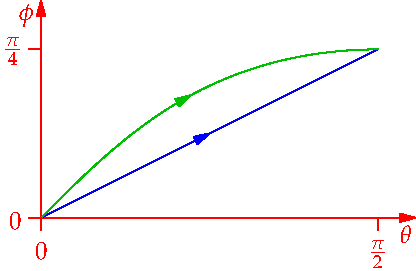
\includegraphics{fund-sphere4} \qquad\qquad
		\href{http://www.math.uci.edu/~ndonalds/math162a/fund-sphere3.html}{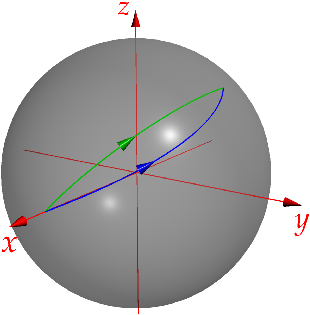
\includegraphics{fund-sphere3}}
	\end{center}
\end{example*}

\goodbreak


If a map of the Earth covers a small latitude range (almost constant $\phi\approx\phi_0$), the first fundamental form is almost similar to a standard dot product $\I\approx (a\cos\phi_0\,\dth)^2+(a\,\D\phi)^2$. If not, say when we travel by plane, the distortion becomes much more apparent.
\begin{center}
	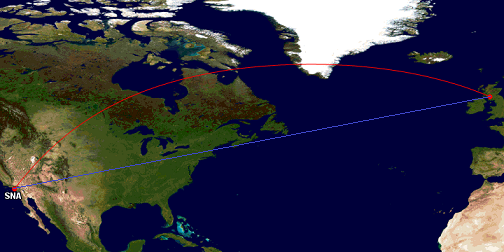
\includegraphics{fund-irvine.png}
\end{center}
The picture shows the \textcolor{red}{\href{http://www.gcmap.com/mapui?P=SNA-PIK}{shortest path}} from Irvine (California) to Irvine (Scotland), as flown by an aircraft in ideal conditions. The \textcolor{blue}{straight line} on the map corresponds to a \emph{longer real-world path.}\smallbreak
If we travel at constant speed, it can be checked that great circles are precisely those curves whose acceleration is entirely in the normal direction. This observation, and its relation to \emph{geodesics} (paths minimizing distance), is a matter for another course.


\begin{example}{}{}
	A skater descends into a paraboloidal bowl $z=\frac 12r^2$ following the path described by $c(t)=(r(t),\theta(t))=(1-t,4t^2)$ in polar co-ordinates. If we parametrize the bowl in polar co-ordinates $\vx(r,\theta)=\bigl(r\cos\theta,r\sin\theta,\frac 12r^2\bigr)$, the fundamental forms are seen to be
	\par
	\begin{minipage}[t]{0.5\linewidth}\vspace{-10pt}
		\begin{gather*}
% 	\vx_r=\threevec{\cos\theta}{\sin\theta}{r},\quad\vx_\theta=\threevec{-r\sin\theta}{r\cos\theta}0,\quad \V U=\frac{1}{\sqrt{1+r^2}}\threevec{-r\cos\theta}{-r\sin\theta}{1},\\
% 	E=1+r^2,\quad F=0,\quad G=r^2,\\
% 	l=\frac{1}{\sqrt{1+r^2}},\quad m=0,\quad n=\frac{r^2}{\sqrt{1+r^2}},\\
			\I=(1+r^2)\,\dr^2+r^2\,\dth^2\\
			\II=\frac 1{\sqrt{1+r^2}}(\dr^2+r^2\,\dth^2)
		\end{gather*}
		For the skater's path, $c'(t)=-\partials r+8t\partials\theta$, whence
		\[
			\I(c',c')=(1+(1-t)^2)+64t^2(1-t)^2
		\]
	\end{minipage}
	\hfill
	\begin{minipage}[t]{0.49\linewidth}\vspace{0pt}
		\flushright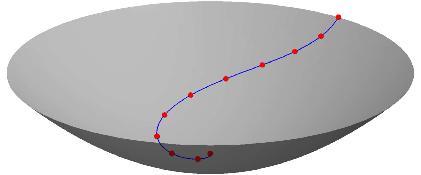
\includegraphics{fund-skater}
	\end{minipage}
	\bigbreak
	The path therefore has arc-length
	\par
	\begin{minipage}[t]{0.6\linewidth}\vspace{-8pt}
		\[
			\int_0^1\sqrt{\I(z',z')}\,\dt =\int_0^1\sqrt{1+(64t^2+1)(1-t)^2}\,\dt \approx 1.82
		\]
		and normal acceleration
		\[
			\vy''\cdot\vn =\II(c',c') =\frac 1{\sqrt{1+(1-t)^2}}\bigl(1+64t^2(1-t)^2\bigr)
		\]
	\end{minipage}
	\hfill
	\begin{minipage}[t]{0.39\linewidth}\vspace{-2pt}
		\flushright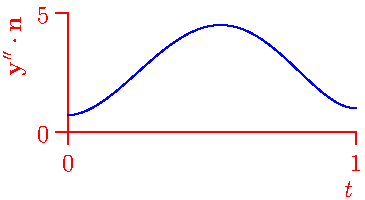
\includegraphics{fund-skater2}
	\end{minipage}
	\medbreak
	By Newton's second law, this is proportional to the component of the force experienced by the skater pushing perpendicularly out from the surface. 
\end{example}

\goodbreak







%\item $\I,\II$ for ruled surface, helicoid?

\begin{exercises}
	\exstart Verify the final details of Example \ref{ex:paraboloidpolar}: that is, compute $\I,\II$ directly using the polar co-ordinate parametrization $\vy(r,\theta)=\bigl(r\cos\theta,r\sin\theta,r^2\big)$.
	
	\begin{enumerate}\setcounter{enumi}{1}  
	  \item\label{exs:revfund} Find the fundamental forms for the surface of revolution $\vx(\theta,v)=\bigl(f(v)\cos\theta,f(v)\sin\theta,v\bigr)$.
	  
	
		\item Compute the first fundamental forms of each parametrized surface wherever they are regular ($a,b,c$ are non-zero constants). Where does each parametrization fail to be regular?\vspace{-2pt}
	  \begin{enumerate}
	    \item Ellipsoid $\vx(\theta,\phi)=(a\cos\theta\cos\phi,b\sin\theta\cos\phi,c\sin\phi)$
	    \item Elliptic paraboloid $\vx(r,\theta)=(ar\cos\theta,br\sin\theta,r^2)$
	    %\item Hyperbolic paraboloid $\vx(u,v)=(au\cosh v,bu\sinh v,u^2)^T$
	    \item Hyperboloid of two sheets $\vx(u,v)=(a\sinh u\cos v,b\sinh u\sin v,c\cosh u)$
	  \end{enumerate}
	  
	  
		\item\label{exs:enneper} Calculate the fundamental forms of Enneper's surface
		\[
			\vx(u,v)=\bigl(u-\tfrac 13u^3+uv^2,v-\tfrac 13v^3+vu^2,u^2-v^2\bigr)
		\]
		
		
		\item Compute $\D\vy$ for the parametrization $\vy(r,\theta)=\bigl(r\cos\theta,r\sin\theta,\sqrt{1-r^2}\bigr)$ of the upper unit hemisphere. Verify that the first fundamental form is the same as in Example \ref{ex:spherepolar2}.
		
	  
	  \item\label{exs:tandevhelix} Let $\vx$ be the tangent developable of a unit speed biregular curve $\vy$ (Exercise \ref*{sec:regularsurfaces}.\ref{exs:tandev}).
	  \begin{enumerate}
	    \item Compute the fundamental forms of $\vx$ in terms of the curvature and torsion of $\vy$.
	    \item If $\vy(u)=\bigl(\cos \frac u{\sqrt 2},\sin\frac u{\sqrt 2},\frac u{\sqrt 2}\bigr)$ is the unit speed helix, show that
	  	\[
	  		\I=\bigl(1+\tfrac{v^2}{4}\bigr)\du^2+2\,\du\dv+\dv^2,\qquad \II=-\tfrac{v}{4}\,\du^2
	  	\]
	 	\end{enumerate}
	 
	  
	  \item Prove that $\II\equiv 0$ if and only if $\vx$ is (part of) a plane.
	
	
		\item Parametrize the great circle in Example \hyperlink{ex:spherepolar4}{\ref*{ex:spherepolar2} (cont)} by $\vz(t)=\bigl(\cos t,{\frac 1{\sqrt 2}\sin t,\frac 1{\sqrt 2}}\sin t\bigr)$, $0\le t\le \frac\pi 2$. Verify that the arc has length $\frac\pi 2$ and that the acceleration of $\vz$ is entirely \emph{normal}; $\vz''=(\vz''\cdot\vn)\vn$.
			
	  
	  \item\label{exs:poincarehalfplane} Equip the upper half plane $y>0$ with the abstract first fundamental form $\I=\smash{\frac 1{y^2}}\bigl(\dx^2+\dy^2\bigr)$. Compare the arc-length between the points $(1,1)$ and $(-1,1)$:
	  \begin{enumerate}
	    \item Over the circular arc $c(t)=\sqrt 2\bigl(\cos t,\sin t\bigr)$ centered at the origin.
	    \item Over the `straight' line $y=1$.
	  \end{enumerate}
	  \emph{This is the Poincaré half-plane model of hyperbolic space. There is neither a surface $\vx:U\to\E^3$ nor a second fundamental form $\II$!}
	  
	  
	  \item (Hard)\lstsp The \emph{torus} obtained by rotating the unit circle in the $x,z$-plane centered at $(2,0,0)$ around the $z$-axis may be parametrized
	  \[
	  	\vx(u,v)=\bigl((2+\cos \phi)\cos\theta,(2+\cos\phi)\sin\theta,\sin\phi\bigr),\quad (\theta,\phi)\in\R^2
	  \]
	  Let $k\neq 0$ be constant and consider the curve $\vy(t)=\vx(kt,t)$ on the torus.
	  \begin{enumerate}
	    \item Prove that $\vy(t)$ has a self-intersection ($\exists s\neq t$ such that $\vy(t)=\vy(s)$) if and only if $k\in\Q$.
	    \item If $k\in\Q$, show that the curve is \emph{periodic} in that there exists a minimum positive $T$ for which $\vy(t+T)=\vy(t)$ for all $t$. Find $T$ in terms of $k$ and write down (don't evaluate!) the integral for the arc-length of the curve over one period.
	  \end{enumerate}
		
	\end{enumerate}
\end{exercises}

\clearpage



\subsection{Principal, Gauss \& Mean Curvatures}\label{sec:principalcurv}

Since $\I$ and $\II$ are symmetric bilinear forms on each tangent space $T_p\R^2$, they may be expressed in matrix form: their matrices with respect to linearly independent vector fields $\vec s,\vec t$ are
\[
	[\I]:=
	\begin{pmatrix}
  	\I(\vec s,\vec s)&\I(\vec s,\vec t)\\
  	\I(\vec s,\vec t)&\I(\vec t,\vec t)
	\end{pmatrix}
	\quad\text{and}\quad
	[\II]:=
	\begin{pmatrix}
  	\II(\vec s,\vec s)&\II(\vec s,\vec t)\\
  	\II(\vec s,\vec t)&\II(\vec t,\vec t)
	\end{pmatrix}\]
	Otherwise said
	\[
		\I\bigl(f\vec s+g\vec t,h\vec s+k\vec t\bigr)=\bigl(f\ g\bigr)[\I]\twovec hk
	\]
	and similarly for $\II$. Matters are simplest when these matrices are \emph{diagonal\ldots}


\begin{defn}{}{curvcoord}
	Linearly independent vector fields $\vec s,\vec t$ are said to be \emph{orthogonal} if $\I(\vec s,\vec t)=0$. They additionally describe \emph{curvature directions} if $\II(\vec s,\vec t)=0$.\smallbreak
	Co-ordinates $u,v$ are \emph{orthogonal}/\emph{curvature-line} if the above apply to the the co-ordinate fields $\partials u,\partials v$.
\end{defn}

In the language of Theorem \ref{thm:fundcoord}, the matrices of the fundamental forms with respect to $\partials u,\partials v$ are 
\[
	A:=
	\begin{pmatrix}
  	E&F\\F&G
	\end{pmatrix}
	\quad\text{and}\quad
	B:=
	\begin{pmatrix}
  	l&m\\m&n
	\end{pmatrix}
	\tag{$\ast$}
\]
Co-ordinates are orthogonal iff $F=\vx_u\cdot\vx_v\equiv 0$ ($\I$ has no $\du\,\dv$ term), and are curvature-line iff $\II$ is also diagonal:
\[
	\I=E\,\du^2+G\,\dv^2\quad\text{and}\quad \II=l\,\du^2+n\,\dv^2
\]
While the meaning of \emph{orthogonal} is clear, the reason for the term \emph{curvature-line} will take a little work.


\begin{examples}{}{}
	\exstart Since the sphere of radius $a$ has $\II=-\frac 1a\I$, any orthogonal co-ordinates on the sphere are curvature-line! E.g., spherical polar co-ordinates: $\I=a^2\bigl(\cos^2\!\phi\,\D\theta^2+\D\phi^2\bigr)$.
	\begin{enumerate}\setcounter{enumi}{1}
	  \item (Example \ref*{sec:fund}.\ref{ex:paraboloidpolar})\lstsp Standard polar co-ordinates are curvature-line for the paraboloid $z=r^2$:
	  \[
	  	\I=(1+4r^2)\,\dr^2+r^2\,\dth^2, \qquad \II=\frac{2}{\sqrt{1+4r^2}}\big(\dr^2+r^2\,\dth^2\bigr)
	  \]
	\end{enumerate}
\end{examples}



\boldinline{A Little Linear Algebra}

The existence of curvature directions is equivalent to the \emph{simultaneous diagonalization} of both matrices ($\ast$). This requires an extension of the concepts of eigenvalues/vectors.


\begin{defn}{}{}
	Let $A,B$ be square matrices of the same dimension. A non-zero vector $\vec v$ is an \emph{eigenvector} of $B$ with respect to $A$ with \emph{eigenvalue} $\lambda$ if
	\[
		(B-\lambda A)\vec v=\vec 0
	\]
\end{defn}

If $A=I$ is the identity matrix, these are standard eigenvalues/vectors. We compute in the usual manner: solve the characteristic polynomial and find $\vec v\in\cN(B-\lambda A)$ in the nullspace\ldots

\goodbreak

\begin{example}{}{simdiag}
	Let $A=\begin{smatrix}2&3\\3&5\end{smatrix}$ and $B=\begin{smatrix}0&1\\1&3\end{smatrix}$.
	\begin{gather*}
		\det(B-\lambda A)=
		\begin{vmatrix}
			-2\lambda&1-3\lambda\\
			1-3\lambda&3-5\lambda
		\end{vmatrix}
		=\lambda^2-1=0\iff \lambda=\pm 1\\
		\vec v_1\in\cN(B-A)=\cN
		\begin{pmatrix}
			-2&-2\\-2&-2
		\end{pmatrix}
		=\Span\twovec 1{-1},\qquad\\
		\vec v_2\in\cN(B+A)=\cN=
		\begin{pmatrix}
			2&4\\4&8
		\end{pmatrix}
		=\Span\twovec 2{-1}
	\end{gather*}
	Note that $\{\vec v_1,\vec v_2\}=\left\{\stwovec{1}{-1},\stwovec 2{-1}\right\}$ is a basis of $\R^2$ consisting of eigenvectors of $B$ with respect to $A$.
\end{example}


\begin{thm}{}{funddiag}
	Let $A,B$ be symmetric matrices of the same dimension, with $A$ \emph{positive-definite.\footnotemark}
	\begin{enumerate}
	  \item There exists a basis of eigenvectors of $B$ with respect to $A$. Moreover, all eigenvalues are \emph{real.}
	  \item If $\vec s,\vec t$ are eigenvectors corresponding to distinct eigenvalues, then $\vec s^TA\vec t=0=\vec s^TB\vec t$.
	\end{enumerate}
\end{thm}

\footnotetext{For all non-zero vectors, $\vec v^TA\vec v>0$. Equivalently, all eigenvalues of $A$ are positive. This means that $\ip{\vec v,\vec w}:=\vec v^TA\vec w$ defines an \emph{inner product} on $\R^n$. In Example \ref{ex:simdiag}, $A$ has eigenvalues $\frac 12(7\pm\sqrt{45})>0$.}


\begin{proof}
\begin{enumerate}
  \item This follows from the famous \emph{spectral theorem} in linear algebra.\footnotemark 
	\item Assume $B\vec s=k_1A\vec s$ and $B\vec t=k_2A\vec t$ where $k_1\neq k_2$, and apply the \textcolor{red}{symmetry} of $A$ and $B$,
	\[
		\left.
		\begin{array}{@{}c@{\,}l}
			\vec s^TB\vec t &=\vec s^T(k_2A\vec t) =k_2\vec s^TA\vec t\\[1pt]
			\textcolor{red}{\parallel}&\\[4pt]
			\vec t^TB\vec s &=\vec t^T(k_1A\vec s) =k_1\vec t^TA\vec s \mathrel{\textcolor{red}{=}}k_1\vec s^TA\vec t
		\end{array}
		\right\}
		\implies (k_2-k_1)\vec s^TA\vec t=0
		\implies \vec s^TA\vec t=0
	\tag*{\qedhere}
	\]
\end{enumerate}
\end{proof}

\footnotetext{In case you're interested:\quad $A$ has an orthogonal eigenbasis $\{\vec x_1,\ldots,\vec x_n\}$ by the spectral theorem. Since its eigenvalues $\mu_i$ are positive, we may scale such that $\Nm{\vec x_i}^2=\frac 1{\mu_i}$. Let $X=(\vec x_1\ \cdots\ \vec x_n)$ so that $X^TAX=I$ is the identity matrix. But then,
\begin{gather*}
\det(B-\lambda A) =\det(X^T)^{-1}\det\bigl(X^TBX-\lambda I\bigr)\det(X^{-1}) =0\iff \det(X^TBX-\lambda I)=0
\end{gather*}
Since $X^TBX$ is symmetric (spectral theorem again), it has an orthogonal eigenbasis $\{\vec w_1,\ldots,\vec w_n\}$ and real eigenvalues $\lambda_k$. Each $\vec v_k:=X\vec w_k$ is an eigenvector of $B$ with respect to $A$ with eigenvalue $\lambda_k$. Since $X$ is invertible, $\{\vec v_1,\ldots,\vec v_n\}$ is a basis.}


%\skip\footins=-\bigskipamount
\boldinline{Application to Surfaces}

With respect to independent vector fields, the matrices $A,B$ of $\I,\II$ are symmetric. Moreover, the regularity of $\vx$ guarantees the positive-definiteness of $A$:
\[
	\forall \vec w\neq\vec 0\implies \vec w^TA\vec w=\I(\vec w,\vec w)=\dvx(\vec w)\cdot\dvx(\vec w)=\Nm{\dvx(\vec w)}^2>0
\]
We may therefore apply Theorem \ref{thm:funddiag} to the matrices of the fundamental forms.

\begin{defn}{}{}
	The \emph{principal curvatures} $k_1,k_2:U\to\R$ of an oriented surface $\vx:U\to\E^3$ are the eigenvalues of $\II$ with respect to $\I$. Corresponding eigenvectors	are \emph{curvature directions.}
	\smallbreak
	The \emph{Gauss} and \emph{mean curvatures} are, respectively, $K:=k_1k_2$ and $H:=\frac 12(k_1+k_2)$.
	\smallbreak
	A point $\vx(p)$ is \emph{umbilic} if $k_1(p)=k_2(p)$.
\end{defn}

%\skip\footins=\bigskipamount

The curvatures are independent of \emph{oriented} co-ordinate changes. If we reverse orientation, then $k_1,k_2$ and $H$ change sign, while $K=k_1k_2$ is unchanged.\smallbreak
At non-umbilic points, Theorem \ref{thm:funddiag} says that curvature directions diagonalize both fundamental forms, in line with Definition \ref{defn:curvcoord}.\smallbreak
At umbilic points, $\II=k\I$ and all directions are curvature directions; any orthogonal directions necessarily diagonalize both fundamental forms. 



\begin{example}{}{totalumbilic}
	Here are two \emph{totally umbilic} surfaces where the curvatures are constant.
	\begin{enumerate}\itemsep2pt
  	\item A plane: \ $\II\equiv 0\implies$ all curvatures are zero.
  	\item A sphere of radius $a$: \ $\II=-\frac 1a\I\implies k_1=k_2= -\frac 1a$, $K=\frac 1{a^2}$ and $H=-\frac 1{a}$.
	\end{enumerate}
	In fact these comprise all totally umbilic surfaces (see Exercise \ref{exs:totallyumbilic}).
\end{example}


\begin{thm}{}{gaussmeancoords}
	\exstart In co-ordinates, the Gauss and mean curvatures are given by
		\[
			K=\frac{ln-m^2}{EG-F^2} =\frac{\det B}{\det A} =\det(A^{-1}B)\quad\text{and} \quad H=\frac{lG+nE-2mF}{2(EG-F^2)}  =\frac 12\tr A^{-1}B
		\]
	\begin{enumerate}\setcounter{enumi}{1}
	  \item At non-umbilic points, the curvatures $k_1,k_2,K,H$ are smooth functions and the curvature directions may be described locally by (smooth) vector fields.
	\end{enumerate}
\end{thm}

\begin{proof}
	\begin{enumerate}
	  \item The principal curvatures are the solutions to the quadratic equation
		\[
			\det\left(
			\begin{pmatrix}
				l&m\\m&n
			\end{pmatrix}
			-\lambda
			\begin{pmatrix}
				E&F\\
				F&G
			\end{pmatrix}
			\right) = (EG-F^2)\lambda^2-(lG+nE-2mF)\lambda+(ln-m^2)
		\]
		of which $K$ and $H$ are the product and half the sum of the roots.
	  \item The roots $\frac{-b\pm\sqrt{b^2-4ac}}{2a}$ of a quadratic are smooth functions of the coefficients unless $b^2-4ac=0$, in which case we have a repeated root ($k_1=k_2$). At non-umbilic points, each eigenspace is one-dimensional, so there is no obstruction to choosing smooth eigenvectors.\footnotemark\qedhere
	\end{enumerate}
\end{proof}

\footnotetext{The impediment to smoothness an umbilic point $\vx(p)$ is that the eigenspace is 2-dimensional so $\lim\limits_{q\to p}\vec v(q)$ need not exist.}


\begin{examples}{}{gaussexs}
	\exstart (Example \ref{ex:paraboloidpolar})\lstsp For the paraboloid $\vx(r,\theta)=\bigl(r\cos\theta,r\sin\theta,r^2\bigr)$, standard polar co-ordinates are curvature-line:
	  \[
	  	A=[\I]=
	  	\begin{pmatrix}
	  		1+4r^2&0\\0&r^2
	  	\end{pmatrix}
	  	\qquad
	  	B=[\II]=
	  	\begin{pmatrix}
	  		\frac 2{\sqrt{1+4r^2}}&0\\
	  		0&\frac{2r^2}{\sqrt{1+4r^2}}
	  	\end{pmatrix}
	  \]
	  The curvatures are therefore
	  \[
	  	k_1=\frac 2{(1+4r^2)^{3/2}}, \quad k_2=\frac 2{\sqrt{1+4r^2}}, \quad K=\frac 4{(1+4r^2)^2}, \quad H=\frac{2+4r^2}{(1+4r^2)^{3/2}}
	  \]
	  The curvatures make sense at the single umbilic point ($r=0$), but the co-ordinates are not curvature-line there since the parametrization fails to be regular ($\vx_\theta(0,\theta)=\V0$).
	  
	\goodbreak
	
	\begin{enumerate}\setcounter{enumi}{1}
	  \item\label{ex:gaussgraph} Parametrize the graph of a function $z=f(x,y)$ in the usual manner $\vx(u,v)=\bigl(u,v,f(u,v)\bigr)$. Then
	  \[
	  	A=[\I]=
	  	\begin{pmatrix}
	  		1+f_u^2&f_uf_v\\
	  		f_uf_v&1+f_v^2
	  	\end{pmatrix}
	  	\qquad
	  	B=[\II]=\frac 1{\sqrt{1+f_u^2+f_v^2}}
	  	\begin{pmatrix}
	  		f_{uu}&f_{uv}\\
	  		f_{uv}&f_{vv}
	  	\end{pmatrix}
	  \]
	  Theorem \ref{thm:gaussmeancoords} tells us that
		\[
			K=\frac{f_{uu}f_{vv}-f_{uv}^2}{(1+f_u^2+f_v^2)^2} \qquad H=\frac{f_{vv}(1+f_u^2)+f_{uu}(1+f_v^2)-2f_uf_vf_{uv}}{2(1+f_u^2+f_v^2)^{3/2}}
		\]
		In the abstract, solving for the curvatures and curvature directions is disgusting. As a sanity check, you should verify that $f(u,v)=u^2+v^2$ recovers exactly the curvatures in the previous example!
	  
		\item\label{ex:tandevgauss} (Exercise \ref*{sec:fund}.\ref{exs:tandevhelix})\lstsp The tangent developable of the unit speed helix has	
	  \[
	  	A=[\I]=
	  	\begin{pmatrix}
	  		1+\tfrac{v^2}{4}&1\\
	  		1&1
	  	\end{pmatrix}
	  	\qquad
	  	B=[\II]=
	  	\begin{pmatrix}
	  		-\tfrac{v}{4}&0\\
	  		0&0
	  	\end{pmatrix}
	  \]
	  The principal curvatures solve
	  \[
	  	\det
	  	\begin{pmatrix}
	  		-\frac v4-\lambda\left(1+\frac{v^2}4\right)&-\lambda\\
	  		-\lambda&-\lambda
	  	\end{pmatrix}
	  	=\frac{v^2}4\lambda^2+\frac v4\lambda=0
	  \]
	  from which 
	  \[
	  	k_1=0,\quad k_2=-\frac 1v,\quad K=0,\quad H=-\frac 1{2v}
	  \]
	  In this case an explicit computation of the curvature directions is not difficult:
	  \begin{gather*}
	  	k_1=0\implies \cN(B-k_1A)=\cN
	  	\begin{pmatrix}
	  		-\frac v4&0\\
	  		0&0
	  	\end{pmatrix}
	  	=\Span\twovec 01\implies \vec s=\partials v\\
	  	k_2=-\frac 1v\implies \cN(B-k_2A)=\cN
	  	\begin{pmatrix}
				\frac 1v&\frac 1v\\
	  		\frac 1v&\frac 1v
	  	\end{pmatrix}
	  	=\Span\twovec 1{-1} \implies \vec t=\partials u-\partials v
	  \end{gather*}
	  where we made the natural choice of vector fields $\vec s,\vec t$. As a sanity check, here are the matrices of the fundamental forms with respect to $\vec s,\vec t$:
	  \begin{align*}
	  	\I(\vec s,\vec s)=\bigl(0\ 1\bigr)A\twovec 01=1,\ \ldots \implies
	  	&[\I]=
	  	\begin{pmatrix}
	  		\I(\vec s,\vec s)&\I(\vec s,\vec t)\\
	  		\I(\vec s,\vec t)&\I(\vec t,\vec t)
			\end{pmatrix}
			=
			\begin{pmatrix}
	  		\textcolor{red}{1}&0\\
	  		0&\textcolor{blue}{\frac{v^2}4}
	  	\end{pmatrix}
	  	\\
	  	&
	  	[\II]=
	  	\begin{pmatrix}
	  		\II(\vec s,\vec s)&\II(\vec s,\vec t)\\
	  		\II(\vec s,\vec t)&\II(\vec t,\vec t)
			\end{pmatrix}
			=
			\begin{pmatrix}
	  		\textcolor{red}{0}&0\\
	  		0&\textcolor{blue}{-\frac{v}4}
	  	\end{pmatrix}
	  \end{align*}
	  in which the principal curvatures are clearly visible:
	  \[
	  	\textcolor{red}{1}k_1=\textcolor{red}{0}, \qquad \textcolor{blue}{\frac{v^2}4}k_2 =\textcolor{blue}{-\frac{v}4}
	  \]
	\end{enumerate}
\end{examples}

\goodbreak

The Gauss and mean curvatures are extremely important quantities for descibing surfaces. Here are a couple of ideas built on these concepts.

\begin{description}
	\item[\normalfont\emph{Minimal Surfaces} $H\equiv 0$:] So-called because they minimize \emph{surface area}: among all surfaces whose boundary is a given closed curve, the surface with minimal surface area has $H\equiv 0$. This is the shape a soap film takes if you dip the curve in soapy water. A minimal surface minimizes the `total tension' of the soap film.
	
\begin{minipage}[t]{0.65\linewidth}\vspace{-9pt}
	More generally, \emph{constant mean curvature} (CMC) surfaces may be used to model soap \emph{bubbles.}
	\item[\normalfont\emph{Constant Gauss Curvature Surfaces}:] Spheres are examples of surfaces of constant positive Gauss curvature. Planes, cones and cylinders are examples of surfaces with $K=0$. A \emph{pseudosphere} with constant $K=-1$ is drawn.
\end{minipage}\hfill\begin{minipage}[t]{0.34\linewidth}\vspace{-20pt}
	\flushright\href{http://www.math.uci.edu/~ndonalds/math162a/curv-pseudosphere.html}{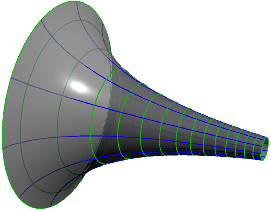
\includegraphics{curv-pseudosphere}}\vspace{-10pt}
\end{minipage}
\end{description}




\boldsubsubsection{Existence of (Curvature-Line) Co-ordinates}

At non-umbilic points, Theorems \ref{thm:funddiag} and \ref{thm:gaussmeancoords} tell us how to find curvature \emph{directions} as vector fields $\vec s,\vec t$. Unfortunately, finding explicit curvature \emph{co-ordinates} is exceptionally unlikely. When you can, it is usually by pure lucky guesswork.

\begin{example*}{\ref*{ex:gaussexs}.\ref{ex:tandevgauss} cont}{}
	Recall that we chose curvature direction fields $\vec s=\partials v$ and $\vec t=\partials u-\partials v$. By inspection, the functions $s=u+v$ and $t=u$ satisfy the required equations:
	\[
		\vec s[s]=1=\vec t[t],\qquad \vec s[t]=0=\vec t[s]
	\]
	It follows that $\vec s=\partials s$ and $\vec t=\partials t$ for curvature-line co-ordinates $s,t$, as you can easily verify using the chain rule. Indeed
	\[
		\I=\frac{v^2}4\,\du^2+\D(u+v)^2 =\ds^2+\frac{v^2}4\,\dt^2,\qquad \II=0\,\ds^2-\frac v4\,\dt^2
	\]
	so that the co-ordinates really do diagonalize both fundamental forms.
\end{example*}

 The simple reason the example is so unlikely is that \emph{mixed partial derivatives must commute}: if $\vec s=\partials s$ and $\vec t=\partials t$ are co-ordinate fields ($\exists s,t:U\to\R$), then their \emph{Lie bracket} (Exercise \ref*{sec:kform}.\ref{exs:liebracketdalpha}) vanishes:
\[
	[\vec s,\vec t]=\left[\partials s,\partials t\right]=\partials s\circ\partials t-\partials t\circ\partials s=0
\]
The astonishing fact is that this simple condition is \emph{locally sufficient.}

\begin{thm}{Co-ordinate fields}{coordfields}
	Let $\vec s,\vec t$ be linearly independent vector fields on $U\subseteq\R^2$.
	\begin{enumerate}
	  \item If there exist functions $s,t:U\to\R$ such that $\vec s=\partials s$, $\vec t=\partials t$, then $[\vec s,\vec t]=0$.
	  \item Suppose $[\vec s,\vec t]=0$ and let $p\in U$. Then there exists a neighborhood $V$ of $p$ and co-ordinate functions $s,t:V\to\R$ for which $\vec s=\partials s,\vec t=\partials t$.
	\end{enumerate}
\end{thm}

We leave a sketch proof of part 2 to Exercise \ref{exs:coordfields}.\smallbreak

\begin{example}{}{}
	The fields $\vec s=\partials x+y\partials y$ and $\vec t=\partials y$ do not arise simultaneously from co-ordinates, since
	\[
		[\vec s,\vec t]=\partials[^2]{x\partial y}+y\partials[^2]{y^2} -\partials[^2]{y\partial x}-\partials y-y\partials[^2]{y^2} =-\partials y\neq 0
	\]
\end{example}

The Lie bracket condition says that explicit co-ordinates corresponding to given vector fields are very unlikely to exist. This is no matter: we typically only need co-ordinates $s,t$ whose fields $\partials s,\partials t$ are \emph{parallel} to $\vec s,\vec t$: that is $\partials s=f\vec s$ and $\partials t=g\vec t$ for some functions $f,g$ (equivalently $\vec s[t]=0=\vec t[s]$). Such co-ordinates do indeed exist, though only \emph{locally,} as shown by one of the most important foundational results in differential geometry.

\begin{thm}{Frobenius}{curvexist}
	Let $\vec s,\vec t$ be linearly independent vector fields on some domain $U$. There exist local co-ordinates $s,t$ whose co-ordinate fields are parallel to $\vec s,\vec t$.\smallbreak
	In particular, if $\vx(p)$ is a non-umbilic point on a surface $\vx:U\to\E^3$, then there exists a neighborhood $V$ of $p$ and curvature-line co-ordinates $s,t$ on $V$.
\end{thm}

Frobenius' theorem comes in many guises and generalizes to higher dimensions, taking the place of Picard's ODE existence/uniqueness theorem (\ref{thm:picard}) for particular classes of PDE. Its proof is far too involved for us, though the informal idea is to search for functions $f,g$ such that $[f\vec s,g\vec t]=0$, a lengthy process that indeed depends on Picard's theorem.




%\begin{proof}

%Let $\vec s$ be a smooth vector field on $U$ with $\vec s_p\neq 0$. Choose any co-ordinates on patch around $p$ such that $\vec s_p=\partialsat{y_1}p$ and write
% \[
% 	\vec s=a\partials{y_1}+b\partials{y_2}\text{ on }V \tag{$b(p)=0$, $a(p)=1$}
% \]
% Shrink neighborhood $V$ (if necessary) such that $a\neq 0$ on $V$. Consider IVP:
% \[
% 	\begin{cases}
% 		\diff[y_2]{y_1}=\frac{b(y_1;y_2)}{a(y_1;y_2)}\\
% 		y_2(0;z_2)=z_2
% 	\end{cases}
% \]
% for any given initial data $\nm{z_2}<\epsilon$. This has a unique solution $y_2=y_2(y_1;z_2)$ defined on $\nm{y_1}<\epsilon$, with initial condition $y_2(0;z_2)=z_2$. Moreover, $y_2$ depends smoothly on $y_1,z_2$. Define $z_1=y_1$, then
% \[
% 	\jacobian{y_1,y_2}{z_1,z_2}\bigr|_{z_1=0}=
% 	\begin{pmatrix}
% 		\partials[y_1]{z_1}&\partials[y_1]{z_2}\\
% 		\partials[y_2]{z_1}&\partials[y_2]{z_2}
% 	\end{pmatrix}
% 	\bigr|_{z_1=0}=
% 	\begin{pmatrix}
% 		1&0\\
% 		\frac ba&\partials[y_2]{z_2}
% 	\end{pmatrix}
% 	\bigr|_{z_1=0}
% 	=
% 	\begin{pmatrix}
% 		1&0\\
% 		0&1
% 	\end{pmatrix}
% \]
% Then $(z_1,z_2)$ are co-ordinates on a neighborhood of $p$. But then
% \[
% 	\vec s=a\partials{y_1}+b\partials{y_2}=a\partials{y_1}+a\diff[y_2]{y_1}\partials{y_2} = a\left[\partials[y_1]{z_1}\partials{y_1}+\partials[y_2]{z_1}\partials{y_2}\right] =a\partials{z_1}
% \]
% Now define $x_1(z_1,z_2):=\int_0^{z_1}\frac{\dt}{a(t,z_2)}$ and $x_2=z_2$. Then $\{x_1,x_2\}$ is a local co-ordinate system for which
% \[
% 	\vec s=a\partials{z_1}=a\partials[x_1]{z_1}\partials{x_1}+a\partials[x_2]{z_1}\partials{x_2} =\partials{x_1}
% \]
% Now use as part of induction step\ldots (YUCK!!!)


%\end{proof}




\goodbreak

%  EXERCISENote also that curvature co-ordinates are non-unique: if $\vec s[t]=0$, then $\vec s\bigl[h(t)\bigr]=h'(t)\vec s[t]=0$ for any function $h:\R\to \R$ with non-zero derivative.



% \begin{aside}
% {\bf Complete surfaces and umbilic points}\ \ A complete surface is a bounded surface which has no edge: e.g., a sphere or an ellipsoid. A complete surface has \emph{genus $g$} if it has $g$ holes: thus the sphere has genus 0 and the torus has genus 1.
% 
% \begin{thm}
% Any complete surface of genus 0 (topologically equivalent to the sphere) has at least one umbilic point.
% \end{thm}
% 
% \begin{proof}[`Proof' - requires topology] Suppose that we have a surface which has no umbilic points. Then at each point we have principal curvatures $k_1>k_2$ and orthogonal principal directions. Making a smooth choice of tangent vector to the surface pointing along the principal direction corresponding to $k_1$ (say) defines a global nowhere-vanishing vector field on the surface. However if the surface is complete and has genus 0, then it is diffeomorphic to the sphere and so we have a non-vanishing vector field on the sphere. This contradicts the hairy ball theorem.
% \end{proof}
% 
% The hairy ball theorem (sometimes called the ``Hairy dog theorem'') says that you cannot comb a hairy ball without there being a cowlick somewhere. Think about smoothly trying to comb down the hair at every point on a sphere: it's impossible, though the proof requires some algebraic topology. Note that a `toriodal dog' can be combed: just comb the hair round the doughnut.
% 
% It is a corollary of the Poincar\'e--Hopf theorem that the only complete surfaces in $\E^3$ which are not required to have an umbilic point are those with genus 1 --- topologically equivalent to the torus.
% \end{aside}


\begin{exercises}{}{}
	\exstart Find the eigenvalues of $B=
	\begin{smatrix}
		-1&-1\\-1&1
	\end{smatrix}$
	with respect to $A=
	\begin{smatrix}
		1&1\\1&2
	\end{smatrix}$.
	If $\vec s,\vec t$ are corresponding eigenvectors, verify that $\vec s^TA\vec t=0=\vec s^TB\vec t$.


\begin{enumerate}\setcounter{enumi}{1}
  \item Parametrize the graph of $x=z^2$; compute $\I,\II$ and the principal, Gauss and mean curvatures.
  
  
  \item Use Theorem \ref{thm:gaussmeancoords} to find the Gauss and mean curvatures of the graph of $y=x^2-z^2$.
  
  
  \item Show that Enneper's surface (Exercise \ref*{sec:fund}.\ref{exs:enneper}) is minimal.
    

  \item\label{exs:tandevcurv} Let $\vx(u,v)=\vy(u)+v\vy'(u)$ be the tangent developable of a unit speed biregular curve $\vy$.
  \begin{enumerate}
    \item Find the principal curvatures, Gauss and mean curvatures of $\vx$.
		\item Compute the curvature directions and find curvature line co-ordinates.
	\end{enumerate}
	(\emph{This is very similar to Example \ref*{ex:gaussexs}.\ref{ex:tandevgauss} - keep track of the changes!})
	
	
	\item With respect to some co-ordinates $u,v$, suppose that a surface has fundamental forms
	\[
		\I=u^2\,\du^2+v^2\,\dv^2,\qquad \II=u^2\,\du^2+2uv\,\du\,\dv+v^2\,\dv^2
	\]
	
	\begin{enumerate}
	  \item Show that the principal curvatures are constant: $k_1=0$ and $k_2=2$.
	  \item Show that $\vec s= v\partials u-u\partials v$ and $\vec t=v\partials u+u\partials v$ are curvature directions.
	  \item Compute the Lie bracket $[\vec s,\vec t]$ to show that these are \emph{not} vector fields with respect to some curvature-line co-ordinates.
	  \item Find explicit curvature-line co-ordinates for the surface; functions $s,t$ such that $\partials s,\partials t$ are \emph{parallel} to $\vec s,\vec t$ and express $\I,\II$ with respect to $s,t$.\par
	  (\emph{Hint: try to guess solutions to $\vec s[t]=0=\vec t[s]$})
	\end{enumerate}
	
	\goodbreak


	\item\label{exs:curvlinerotation} Rotate $y=f(x)$ around the $x$-axis and parametrize the surface via
	\[
		\vx(\phi,v)=\bigl(v,f(v)\cos\phi,f(v)\sin\phi\bigr)
	\]
	\begin{enumerate}
	  \item Verify that the co-ordinates $\phi,v$ are curvature-line, compute the principal curvatures, and show that the Gauss and mean curvatures are
		\[
			K=-\frac{f''(v)}{f(v)\bigl(1+f'(v)^2\bigr)^2}\qquad H=\frac{f(v)f''(v)-1-f'(v)^2}{2f(v)\bigl(1+f'(v)^2\bigr)^{3/2}}
		\]
		\item Demonstrate the following by choosing suitable $f(v)$:
		\begin{enumerate}
		  \item A cylinder has $K=0$;
		  \item A cone has $K=0$;
		  \item A sphere of radius $a$ has $K=\frac 1{a^2}$.
		  \item A \emph{catenoid} $f(v)=a^{-1}\cosh(av-c)$ is a minimal surface.
		\end{enumerate}

	  \item Suppose $\vx$ is a minimal surface $H\equiv 0$. By writing $g(v)=1+\bigl(f'(v)\bigr)^2$, show that
	  \[
	  	1+f'^2=g^2=a^2f^2
	  \]
	  for some constant $a$. By making the substitution $f(v)=a^{-1}\cosh\bigl(ah(v)\bigr)$ for some unknown function $h(v)$, show that the surface is a \emph{catenoid.}
	  
	  \item Plainly $K\equiv 0$ if and only if $f''(v)\equiv 0$. What are these surfaces? More generally, if the surface has constant non-zero Gauss curvature $K$, show that $f$ satisfies a non-linear ODE
	  \[
	  	Kf^2=(1+f'^2)^{-1}+c
	  \]
	  for some constant $c$\quad (\emph{solving for $f$ requires an elliptic integral when $c\neq 0$, so don't try!}).
	\end{enumerate}
	
	
	\item The \emph{tractrix} is parametrized by $\vy(t)=\bigl(\sinh^{-1}t-t(1+t^2)^{-1/2}, (1+t^2)^{-1/2}\bigr)$. By revolving this curve around the $x$-axis, show that the resulting surface is a pseudosphere with $K\equiv -1$.
	
	
  \item We know that the Gauss and mean curvature are defined in terms of the principal curvatures. By writing down a suitable quadratic polynomial, prove that knowing of $H,K$ is sufficient to recover the principal curvatures.
	
	  
  \item The graph of a function $z=f(x,y)$ is parametrized by $\vx(u,v)=\bigl(u,v,f(u,v)\bigr)$. What can you say about the surface if $(u,v)$ are curvature-line co-ordinates?\par
  (\emph{Hint: recall Example \ref{ex:paraboloidpolar}})
  
  
  \item\label{exs:curvforms} Suppose $u,v$ are curvature-line co-ordinates for a surface $\vx$. Explain why $\vn_u=-k_1\vx_u$ and $\vn_v=-k_2\vx_v$.


	\item\label{exs:totallyumbilic} Suppose that a surface $\vx:U\to\E^3$ is totally umbilic $\II=k\I$ for some function $k:U\to\R$.
	\begin{enumerate}
	  \item Use Exercise \ref{exs:curvforms} and $\vn_{uv}=\vn_{vu}$ to prove that $k$ is constant.
	  \item Prove that $\vx$ is (part of) a plane or a sphere (recall Example \ref{ex:totalumbilic}).\par
	  (\emph{Hint: If $k\neq 0$ consider $\vc:=\vx+\frac 1k\vn$\ldots})
	\end{enumerate}


	\item\label{exs:coordfields} We prove part 2 of Theorem \ref{thm:coordfields}. Given the assumptions, define the \emph{dual 1-forms} to $\vec s,\vec t$:
  \[
  	\alpha(\vec s)=1=\beta(\vec t) \quad\text{and}\quad \alpha(\vec t)=0=\beta(\vec s)
  \]
  Use Exercise \ref*{sec:kform}.\ref{exs:liebracketdalpha} to prove that $\D\alpha=0=\D\beta$. Hence conclude  (footnote, page \pageref{fn:poincare}) that (locally) $\alpha=\ds$ and $\beta=\dt$ for some functions $s,t$.

\end{enumerate}
\end{exercises}

\clearpage



\subsection{Power Series Expansions and Euler's Theorem}\label{sec:eulersthm}

In this section we intersect a surface with certain planes and consider the resulting curves. The curvatures provide data about these curves and thus tell us something about the local shape of the surface. The key is to see how curvatures describe a quadratic approximation to a surface.\par

\begin{minipage}[t]{0.63\linewidth}\vspace{0pt}
At a regular point $P$ on a surface $S$, choose axes such that $P$ is the origin and the $(x,y)$-plane is tangent\footnotemark{} to $S$. By Theorem \ref{thm:implicit}, $S$ is locally the graph of a function $z=f(x,y)$, which we may parametrize in the usual manner
\[\vx(u,v)=\bigl(u,v,f(u,v)\bigr)\]
\end{minipage}\hfill\begin{minipage}[t]{0.36\linewidth}\vspace{0pt}
	\flushright\href{http://www.math.uci.edu/~ndonalds/math162a/euler-setup.html}{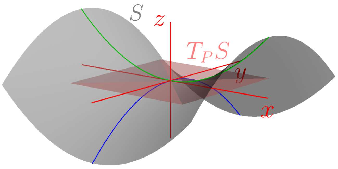
\includegraphics{euler-setup}}
\end{minipage}\par

\footnotetext{This amounts to applying a rigid motion (direct isometry) to the surface, which does nothing to the fundamental forms.}

The unit normal vector $\vn_P=\vk$ is therefore the standard vertical basis vector. Since the tangent plane at $P$ is the $(x,y)$-plane, we see that $f_u(0,0)=0=f_v(0,0)$; substituting into Example \ref{ex:paraboloidpolar} yields the fundamental forms \emph{at $P$}:
\begin{gather*}
\begin{array}{@{}l}
\I_{P}=\du^2+\dv^2\\[4pt]
\II_{P}=f_{uu}\,\du^2+2f_{uv}\,\du\dv+f_{uv}\,\dv^2
\end{array}
\qquad
[\I]_{P}=\begin{pmatrix}
1&0\\0&1
\end{pmatrix}\qquad [\II]_P=\Hess f=\begin{pmatrix}
		f_{uu}&f_{uv}\\
		f_{uv}&f_{vv}
	\end{pmatrix}
\end{gather*}
The last matrix is the \emph{Hessian} of $f$, and the Gauss and mean curvatures at $P$ are
\[K(P)=\det\Hess f(0,0)\quad\text{and}\quad H(P)=\frac{1}{2}\tr\Hess f(0,0)\]
It bears repeating that these expressions are only valid \emph{at the origin} $O\in U$ (equivalently $P\in S$). Although the co-ordinates $u,v$ will extend nearby on the surface, the first fundamental form need not be diagonal anywhere except at the origin.\smallbreak

Now suppose we rotate the $(x,y)$-plane so that the axes point in the principal directions. Then the Hessian is also diagonal ($f_{uv}(0,0)=0$) and the principal curvatures at $P$ are
\[k_1=f_{uu}(0,0)\quad\text{and}\quad k_2=f_{vv}(0,0)\]

\begin{thm}{}{taylor2}
If the graph of $z=f(x,y)$ is tangent to the $(x,y)$-plane at the origin $O$ so that the axes are the curvature directions, then the Maclaurin approximation of the function $f(x,y)$ is
\begin{align*}
f(x,y)&\approx f(O) +(x\ y)\at{\nabla f}{O} +\frac 12(x\ y)\Hess f(O)\twovec{x}{y} +\text{ higher order terms}\\
% &=f(O) +(x\ y)\twovec 00 +\frac 12(x\ y)
% \begin{pmatrix}
%        k_1&0\\
%        0&k_2
%       \end{pmatrix}\twovec{x}{y} +\text{ higher order terms}\\
&=\frac{1}{2}k_1(O)x^2+\frac{1}{2}k_2(O)y^2+\text{ higher order terms}\tag*{\qedhere}
\end{align*}
\end{thm}


\begin{example}{}{hypparabeuler}
Let $f(x,y)=x^2-y^2$ (above picture). At the origin, $\vx(u,v)=\bigl(u,v,u^2-v^2\bigr)$ has
\[\I=\du^2+\dv^2,\quad \II=2(\du^2-\dv^2),\quad k_1=2,\quad k_2=-2,\quad K=-4,\quad H=0\]
In this case the Maclaurin approximation is exact!
\[\frac 12k_1x^2+\frac 12k_2y^2=x^2-y^2=f(x,y)\]
\end{example}

\goodbreak

\boldsubsubsection{Level Curves: intersections with planes parallel to the tangent plane}

If $c$ is small, then the intersection of $S$ with a plane $c\vn_P+T_PS$ parallel to the tangent plane is a \emph{level curve}; in our analysis, they correspond to level curves $f(x,y)=$ constant. Theorem \ref{thm:taylor2} tells us how level curves depend on the curvatures. For instance, if $k_1,k_2$ have opposite signs, then for small $c$,
\[k_1x^2+k_2y^2\approx 2c\]
is approximately a \emph{hyperbola.}

\begin{defn}{}{pointtype}
Suppose $k_1,k_2,K,H$ are the curvatures of a surface $S$ at a point $P$. We say that $P$ is:
\begin{description}\itemsep0pt
	\item[\normalfont\emph{Elliptic}]\negthickspace$\iff K>0\iff k_1,k_2\neq 0$ and have the same sign.\\
  Level curves near $P$ are approximately \emph{ellipses.}
  \item[\normalfont\emph{Hyperbolic}]\negthickspace$\iff K<0\iff k_1,k_2\neq 0$ and have opposite signs.\\
  Level curves near $P$ are approximately \emph{hyperbolæ.}
  \item[\normalfont\emph{Parabolic}]\negthickspace$\iff K=0$ and $H\neq 0 \iff$ exactly one of $k_1,k_2$ is zero.\\
  Level curves near $P$ are approximately a pair of \emph{parallel lines}, e.g.\ $x=\pm c$.
  \item[\normalfont\emph{Planar}]\negthickspace$\iff K=H=0\iff k_1=k_2=0$.\\
  The curvatures provide no data as to the level curves near $P$.
\end{description}
\end{defn}


\begin{example*}{\ref{ex:hypparabeuler}, mk.\,II}{}
For the graph of $z=x^2-y^2$, the level curve $x^2-y^2=c\neq 0$ is a hyperbola.\par
\begin{minipage}[t]{0.63\linewidth}\vspace{-5pt}
In fact this is true everywhere on this surface: under the usual parametrization $\vx(u,v)=\bigl(u,v,u^2-v^2\bigr)$, we have
\[K=-\frac{4}{(1+4u^2+4v^2)^2}\quad\text{and}\quad  H=\frac{4(v^2-u^2)}{(1+4u^2+4v^2)^{3/2}}\]
Since $K<0$ everywhere, all points are hyperbolic.
\end{minipage}\hfill\begin{minipage}[t]{0.36\linewidth}\vspace{0pt}
\flushright\href{http://www.math.uci.edu/~ndonalds/math162a/euler-setup3.html}{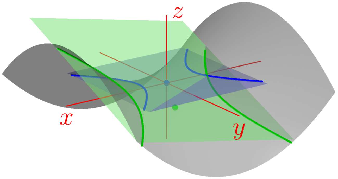
\includegraphics{euler-setup3}}
\end{minipage}\smallbreak
In the picture, shifted tangent planes $c\vn_P+T_PS$ and their intersections with the surface are drawn for two points. In both cases the level curves are genuine hyperbolæ.
\end{example*}



\boldsubsubsection{Normal Curvature: intersections with planes containing the normal vector}

Theorem \ref{thm:taylor2} is the surface analogy of Exercise \ref*{sec:radii}.\ref{exs:curvetaylor}: a regular curve in $\E^2$ passing through the origin horizontally at $t=0$ has its graph given locally by
\[y=\frac 12\kappa(0)x^2+\text{higher order terms}\tag{$\ast$}\]
We put this to work by considering the curvature of curves passing through a point on a surface.

\begin{defn}{}{}
Let $S$ be a surface and $\vv_P\in T_PS$ a non-zero tangent vector.\smallbreak
The \emph{normal curvature} $\nu(\vv_P)$ is the curvature at $P$ of the curve\footnotemark{} $S\cap\Span\{\vv_P,\vn_P\}$.\smallbreak
We say that $\vv_P$ is \emph{asymptotic} if $\nu(\vv_P)=0$.
\end{defn}

\footnotetext{The curve is the \emph{connected component} of $S\cap\Span\{\vv_P,\vn_P\}$ containing $P$.}

\goodbreak

The normal curvature is surprisingly easy to compute.

\begin{thm}{Euler}{}
Suppose $\vv_P$ makes angle $\psi$ with the first principal curvature direction. Then %the %normal curvature of $S$ in the direction $\vv_P$ is
\[\nu(\vv_P)=k_1\cos^2\psi +k_2\sin^2\psi\]
Moreover, the principal curvatures are the extremes of $\nu(\vv_P)$: e.g.\ if $k_1\le k_2$, then
\[k_1\le\nu(\vv_P)\le k_2\]
\end{thm}

\begin{proof}
Choose axes such that the principal curvature directions at $P$ are $\vi,\vj$, and the unit normal is $\vn_P=\vk$. The surface is locally the graph of a function $z=f(x,y)$ satisfying Theorem \ref{thm:taylor2}. If $(r,\psi)$ are standard polar co-ordinates on the $(x,y)$-plane, then 
	\begin{align*}
		z&=\tfrac{1}{2}k_1(r\cos\psi)^2+\tfrac{1}{2}k_2(r\sin\psi)^2+\cdots= \frac 12(k_1\cos^2\psi+k_2\sin^2\psi)r^2+\cdots
	\end{align*}
Now fix $\psi$. Without loss of generality, we may assume $\vv_P$ has unit length since only its direction matters. Our curve of interest $\vy_P\subset\Pi(\vv_P)$ may be parametrized
	\[\vy(r)= r\vv_P+f(r\cos\psi,r\sin\psi)\,\vn_P= \threevec{r\cos\psi}{r\sin\psi}{f(r\cos\psi,r\sin\psi)}=\threevec{r\cos\psi}{r\sin\psi}{\frac 12\nu r^2+\cdots}
	\]
	The last equality used observation ($\ast$), where $\nu$ is the normal curvature. Compare the $z$-expressions for the main result. For the final observation, note that
	\[\nu=k_1+(k_2-k_1)\sin^2\phi\in[k_1,k_2]\tag*{\qedhere}\]
\end{proof}

% \begin{example*}[lower separated=false, sidebyside, sidebyside align=top seam, sidebyside gap=0pt, righthand width=0.36\linewidth]{\ref{ex:hypparabeuler}, mk.\,III}{}
% For the graph of $z=x^2-y^2$, if $\psi=\frac{5\pi}6$, then
% \begin{align*}
% \nu&=2\cos^2\frac{5\pi}6-2\sin^2\frac{5\pi}6= 2\left[\left(\frac{\sqrt 3}2\right)^2-\left(\frac 1{\sqrt 3}\right)^2\right] =\frac 56
% \end{align*}
% \tcblower
% \flushright	\flushright\href{http://www.math.uci.edu/~ndonalds/math162a/euler-setup2.html}{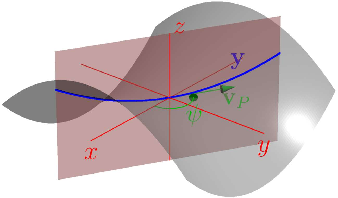
\includegraphics{euler-setup2}}
% \end{example*}


\begin{examples}{}{}
\exstart If $P$ is a planar point, then all normal curvatures are zero and all directions are asymptotic.
\begin{enumerate}\setcounter{enumi}{1}
\begin{minipage}[t]{0.6\linewidth}\vspace{0pt}
  \item For the graph of the hyperbolic paraboloid $z=x^2-y^2$ (Example \ref{ex:hypparabeuler}) at the origin, if $\psi=\frac{5\pi}6$, then
	\[
	\nu(\vv_O)=2\cos^2\frac{5\pi}6-2\sin^2\frac{5\pi}6=\frac 32-\frac 23=\frac 56 %2\left[\left(\frac{\sqrt 3}2\right)^2-\left(\frac 1{\sqrt 3}\right)^2\right] =\frac 56
	\]
	Indeed since every point is hyperbolic, there are always two asymptotic directions at each point: these correspond to the angles $\psi\in(-\frac\pi 2,\frac\pi 2)$ for which 
	\[k_1\cos^2\psi+k_2\sin^2\psi=0\iff \tan\psi=\pm\sqrt{-\frac{k_1}{k_2}}\]
\end{minipage}\hfill\begin{minipage}[t]{0.39\linewidth}\vspace{0pt}
  \flushright	\flushright\href{http://www.math.uci.edu/~ndonalds/math162a/euler-setup2.html}{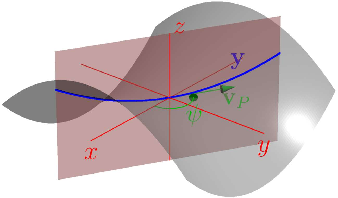
\includegraphics{euler-setup2}}
\end{minipage}\par

  \item A elliptic paraboloid $z=x^2+y^2$ has no asymptotic directions at any point. In its usual parametrization, the principal curvatures are both positive everywhere and  the normal curvature at an point is therefore $\vn(\vv_P)=k_1\cos^2\theta+k_2\sin^2\theta>0$.

%   \item in the third example, there are only asymptotic directions at the parabolic points when $v=0$. These point parallel to the $y$-axis.
\end{enumerate}
\end{examples}

\goodbreak

\boldsubsubsection{The Second Fundamental Form and the Local Shape of a Surface}

Part of our standard approach is to transfer calculations and analysis on surfaces to the parametrization space. By appealing to the ideal of \emph{normal acceleration} (Theorem \ref{thm:fundformcurves}), we may easily transfer the notion of an asymptotic vector to a property of the second fundamental form.

\begin{thm}{}{asymptoticvec}
Suppose $\vx:U\to\E^3$ is an oriented surface and let $\vec w_p\in T_p\R^2$ be a non-zero tangent vector. Then $\dvx(\vec w_p)$ is asymptotic iff $\II(\vec w_p,\vec w_p)=0$.
\end{thm}

We tend to call such a tangent vector $\vec w_p$ asymptotic in its own right.\smallbreak

We can moreover restate the point-types introduced in Definition \ref{defn:pointtype} by introducing a related object.

\begin{defn}{}{}
The \emph{Dupin indicatrix} at $p\in U$ is the set of tangent vectors $\vec w_p\in T_p\R^2$ such that $\II(\vec w_p,\vec w_p)=\pm 1$.
\end{defn}

If $\vec s_p,\vec t_p$ are orthonormal\footnote{I.e.\ $\I(\vec s_p,\vec s_p)=1=\I(\vec t_p,\vec t_p)$ and $\I(\vec s_p,\vec t_p)=0$.} curvature directions and $\vec w_p=a\vec s_p+b\vec t_p$, then the Dupin indicatrix has equation
\begin{align*}
\II(\vec w_p,\vec w_p)&=a^2\II(\vec s_p,\vec s_p) +2ab\II(\vec s_p,\vec t_p) + b^2\II(\vec t_p,\vec t_p) =k_1a^2+k_2b^2=\pm 1
\end{align*}
This defines a curve in the tangent space $T_p\R^2$ whose type depends on the signs of the principal curvatures. In essence, the Dupin indicatrix is a depiction of the level curves obtained by taking the intersection $S\cap (c\vn_P+T_PS)$ for \emph{infinitesimal} $c$; unlike real level curves, the indicatrix is an genuine conic! We summarize all possibilities in a table.
\begin{center}
\begin{tabular}{c|c|c}
type of point&\# of asymptotic directions&Dupin indicatrix\\\hline
elliptic&0&ellipse\\
hyperbolic&2&pair of hyperbolæ\\
parabolic&1&pair of parallel lines\\
planar&$\infty$&empty
\end{tabular}
\end{center}
The advantage of this approach is that it is co-ordinate independent: $\II(\vec w_p,\vec w_p)=\pm 1$ describes the same \emph{type} of curve regardless of which basis vectors/co-ordinates one uses to evaluate $\II$.


\begin{examples}{}{}
For a parametrized surface $\vx$, at a given point $p=(u_0,v_0)$, write $\vec w_p=a\partialsat up+b\partialsat vp$.
\begin{enumerate}
  \item The tangent developable of the unit speed helix has
	\[\II(\vec w_p,\vec w_p)=-\frac{v_0}4\,\du^2(\vec w_p,\vec w_p)=-\frac{v_0}4a^2\]
	The single asymptotic direction is $\vec w_p=\smash{\partialsat vp}$, the direction of zero curvature. The Dupin indicatrix is a pair of parallel lines
	\[-\frac{v_0}4a^2=\pm 1\implies \vec w_p=\pm\frac 2{\sqrt{\nm{v_0}}}\partialsat up+b\partialsat vp\]
	
\begin{minipage}[t]{0.75\linewidth}\vspace{0pt}
	\item The graph of the surface $z=x^2y$ has second fundamental form
	\[\II=\frac{2}{\sqrt{1+4u^2v^2+u^4}}\bigl(v\,\du^2+2u\,\du\dv\bigr)
	\]
	At the point $p=(1,2)$ (i.e.\ $\vx(p)=(1,2,2)$), we see that
	\[\II(\vec w_p,\vec w_p)=\frac 4{\sqrt{10}}\bigl(a^2+ab\bigr)=\frac 4{\sqrt{10}}a(a+b)\]
	The point is hyperbolic with \textcolor{Green}{asymptotic directions} $\partialsat vp$ and $\partialsat up-\partialsat vp$ (corresponding to $a=0$ and $a+b=0$). The \textcolor{blue}{indicatrix} comprises the two hyperbolæ $a(a+b)=\pm\frac{\sqrt 10}4$.
\end{minipage}\hfill\begin{minipage}[t]{0.24\linewidth}\vspace{0pt}
	\flushright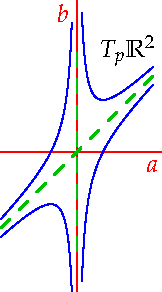
\includegraphics{euler-indicatrix}
\end{minipage}
\end{enumerate}
\end{examples}


\begin{exercises}{}{}
\exstart Consider the graph of the function $z=x^2-3y^2+7xy^3+9y^4$.
\begin{enumerate}\setcounter{enumi}{1}
  \item[]\begin{enumerate}
  	\item Find the Gauss and mean curvatures at the origin.
  	\item Find the normal curvature at the origin for the curve in the surface described by $x=y$.
  \end{enumerate}
  
  
  \item For the elliptic paraboloid $z=x^2+y^2$, let $P=(1,2,5)$ be a fixed point.
  \begin{enumerate}
    \item Find the maximum and minimum values for the normal curvature at $P$.
    \item Find the Dupin indicatrix at $P$.
  \end{enumerate}
  
  
  \item For the hyperbolic paraboloid $z=x^2-y^2$, let $p=(u_0,v_0)$ and $P=\bigl(u_0,v_0,u_0^2-v_0^2\bigr)$. If $c\neq 0$, prove that the intersection of the parallel plane $c\vn_P+T_PS$ with the paraboloid may be expressed
  \[(x-u_0)^2-(y-v_0)^2=\text{constant},\quad z=x^2-y^2\]
  That is, the level curves really are hyperbolæ.


	\item Consider the graph of the surface $z=x^2+y^4$.
	\begin{enumerate}
	  \item Compute the Gauss curvature and classify all points according to Definition \ref{defn:pointtype}.
	  \item Sketch the level curves $z=c$ where $c=1$, $\frac 1{100}$ and $\frac 1{10000}$ and compare these to the Dupin indicatrix at the origin.\par
	  (\emph{This should convince you of the importance that $c$ be small!})
	\end{enumerate}
	
	
	\item Prove Theorem \ref{thm:asymptoticvec} by considering the normal acceleration of the curve $S\cap\Span\{\vv_P,\vn_P\}$.
	
\end{enumerate}
\end{exercises}


\clearpage




\subsection{Adaptive Frames \& Gauss' Remarkable Theorem}

We repurpose an idea first encountered when studying curves. 

\begin{defn}{}{adaptiveframe}
Let $\vx:U\to\E^3$ parametrize a surface $S=\vx(U)$. A \emph{moving frame} for $S$ is a triple of smooth functions $\ve_1,\ve_2,\ve_3$ on $U$ such that, for each $p\in U$,
\begin{quote}
$\bigl\{\ve_1(p),\ve_2(p),\ve_3(p)\bigr\}$ is a positively oriented orthonormal basis of $T_{\vx(p)}\E^3$
\end{quote}
If $S$ is oriented, we say that a frame is \emph{adaptive} if $\ve_3=\vn$ is the unit normal field.
\end{defn}

For an adaptive frame, the tangent plane at each point is $T_{\vx(p)}S=\Span\{\ve_1(p),\ve_2(p)\}$.\par
We will often refer to the matrix-valued function $\cE=\bigl(\ve_1\ \ve_2\ \ve_3\bigr):U\to\rSO_3(\R)$ as the frame.

\begin{examples}{}{adaptive}
We'll repeatedly analyze three examples through this section.
\begin{enumerate}\itemsep0pt
  \item The parabolic cylinder $\vx(u,v)=\bigl(u,v,\frac 12u^2\bigr)$ has an adaptive frame
	\[
	\textcolor{red}{\ve_1}=\frac 1{\sqrt{1+u^2}}\threevec 10u\qquad \textcolor{blue}{\ve_2}=\threevec 010\qquad \textcolor{Green}{\ve_3}=\frac 1{\sqrt{1+u^2}}\threevec{-u}01
	\]
	\item The sphere of radius $R$ in spherical polar co-ordinates $\vx(\psi,\phi)$ has an adaptive frame\footnotemark
	\[
	\textcolor{red}{\ve_1}=\threevec{-\sin\psi}{\cos\psi}0\qquad \textcolor{blue}{\ve_2}=\threevec{-\cos\psi\sin\phi}{-\sin\psi\sin\phi}{\cos\phi}\qquad \textcolor{Green}{\ve_3}=\vx=\threevec{\cos\psi\cos\phi}{\sin\psi\cos\phi}{\sin\phi}
	\]
	\item The paraboloid $\vx(r,\psi)=\bigl(r\cos\psi,r\sin\psi,\frac 12r^2\bigr)$ has an adaptive frame
	\[
	\textcolor{red}{\ve_1}=\frac 1{\sqrt{1+r^2}}\threevec{\cos\psi}{\sin\psi}{r}\qquad \textcolor{blue}{\ve_2}=\threevec{-\sin\psi}{\cos\psi}0\qquad \textcolor{Green}{\ve_3}=\frac 1{\sqrt{1+r^2}}\threevec{-r\cos\psi}{-r\sin\psi}1
	\]
\end{enumerate}
%\hangindent0pt\relax
In the pictures we've reduced the lengths of the frame vectors for clarity.
	\begin{center}
	\href{http://www.math.uci.edu/~ndonalds/math162a/moving-paracyl.html}{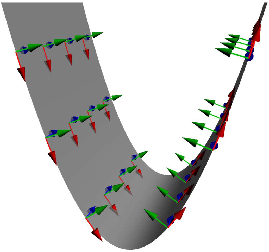
\includegraphics[scale=0.9]{moving-paracyl}}
	\quad
	\href{http://www.math.uci.edu/~ndonalds/math162a/moving-sphere.html}{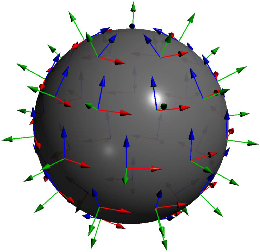
\includegraphics[scale=0.9]{moving-sphere}}
	\quad
	\href{http://www.math.uci.edu/~ndonalds/math162a/moving-paraboloid.html}{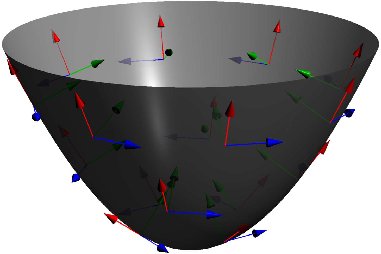
\includegraphics[scale=0.85]{moving-paraboloid}}
	\end{center}
In each case the first two vectors were obtained by differentiating with respect to the co-ordinates (and normalizing if necessary). This only works because all these co-ordinate systems are \emph{orthogonal}!
\end{examples}


% 	\href{http://www.math.uci.edu/~ndonalds/math162a/moving-cylinder.html}{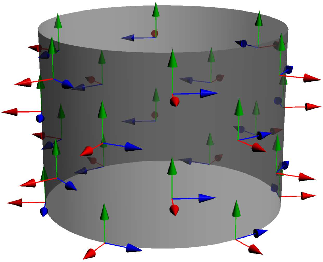
\includegraphics{moving-cylinder}}


\skip\footins=-1.5\bigskipamount
\footnotetext{We use $\psi$ instead of $\theta$ since we'll need the latter for something else in a moment\ldots}
\skip\footins=\bigskipamount
\vfil
\goodbreak

As with the Frenet frame, our strategy is to treat the analysis of a surface $\vx:U\to\E^3$ two stages:
\begin{enumerate}
  \item Describe how $\vx$ moves with respect to the frame.
  \item Describe how the frame itself moves. 
\end{enumerate}
As we're now used to, we describe infinitesimal change using 1-forms, following an approach pioneered by Élie Cartan around 1899.

\begin{defn}{}{mcforms}
Let $\vx:U\to\E^3$ be a smooth map and $\cE=(\ve_1\ \ve_2\ \ve_3)$ a moving frame. The \emph{metric forms} $\theta_j$ and the \emph{connection forms} $\omega_{jk}$ are the 1-forms on $U$ defined by
\[\theta_j:=\ve_j\cdot\dvx,\quad \omega_{jk}=\ve_j\cdot\D\ve_k\]
where $j,k\in\{1,2,3\}$.
\end{defn}

Since $\ve_1,\ve_2,\ve_3$ are orthonormal, these forms are simply the co-ordinates of $\dvx$, $\D\ve_1$, $\D\ve_2$, $\D\ve_3$ with respect to the moving frame:
\[\dvx=\sum_{j=1}^3(\ve_j\cdot\dvx)\ve_j=\ve_1\theta_1+\ve_2\theta_2+\ve_3\theta_3,\qquad \D\ve_k=\sum_{j=1}^3\ve_j\omega_{jk}\tag{$\ast$}\]
If the frame is adaptive, then $\theta_3=0$. Moreover, for any frame, there are only three independent connection forms.

\begin{lemm}{}{}
For all $j,k$, we have $\omega_{jk}=-\omega_{kj}$. In particular $\omega_{jj}=0$.
\end{lemm}

\begin{proof}
Apply $\D$ to the identity $\ve_j\cdot\ve_k=0$ or 1 to see that
\[0=\D\ve_j\cdot\ve_k+\ve_j\cdot\D\ve_k=\omega_{kj}+\omega_{jk}\tag*{\qedhere}\]
\end{proof}

If ($\ast$) are arranged in matrix format, the subscripts follow the usual row/column convention:
\[\dvx=\bigl(\ve_1\ \ve_2\ \ve_3\bigr)\threevec{\theta_1}{\theta_2}{\theta_3}=\cE\Theta,\qquad \D \cE=\bigl(\ve_1\ \ve_2\ \ve_3\bigr)
	\begin{pmatrix}
		0&\omega_{12}&\omega_{13}\\
		-\omega_{12}&0&\omega_{23}\\
		-\omega_{13}&-\omega_{23}&0
	\end{pmatrix}
	=\cE\lomega\]
	The second expression should remind you of the Frenet-Serret equations for a curve! The metric forms get their name because they \emph{measure} small changes on the surface. The connection forms tell us how nearby frames are related (\emph{connected}): if $\vec s_p\in T_p\R^2$, then
% \[\ve(p+\vec s)\approx \ve_1(p)+\D\ve_1(\vec s_p)=\ve_1(p)+\sum_{j=2}^3\ve_j\omega_{jk}(\vec s)\]
\[\cE(p+\vec s_p)-\cE(p)\approx \D \cE(\vec s_p)=\cE\lomega(\vec s_p)\]
The fundamental forms of $\vx$ can be written in terms of $\Theta$ and $\lomega$; in an adaptive frame this is particularly simple.

\begin{lemm}{}{iadaptiveframe}
In an adaptive frame
\[\I=\dvx\cdot\dvx=\theta_1^2+\theta_2^2\quad\text{and}\quad \II=-\dvx\cdot\D\ve_3=-\theta_1\omega_{13}-\theta_2\omega_{23}\]
\end{lemm}

\begin{examples*}{\ref{ex:adaptive}, mk.\,II}{}
You needn't compute all exterior derivatives $\D\ve_k$; use the skew-symmetry of $\lomega$ to help and look for which frame fields are easier to differentiate! The expressions for the fundamental forms should be a sanity check, since we know how to compute them already.
	\begin{enumerate}
	  \item The parabolic cylinder has
  	\begin{align*}
  	\dvx=\threevec 10u\du+\threevec 010\dv=\sqrt{1+u^2}\ve_1\,\du+\ve_2\,\dv
  	&\implies \theta_1=\sqrt{1+u^2}\,\du,\ \ \theta_2=\dv\\[-4pt]
  	&\implies \I=(1+u^2)\,\du^2+\dv^2
  	\end{align*}
  	Since $\ve_2$ is constant, we have $\D\ve_2=\V0$ from which
  	\[\omega_{12}=\ve_1\cdot\D\ve_2=0,\quad \omega_{23}=-\omega_{32}=-\ve_3\cdot\D\ve_2=0\]
  	The final connection form requires a derivative:
  	\[\omega_{13}=\ve_1\cdot\D\ve_3=\frac 1{\sqrt{1+u^2}}\threevec 10u\cdot\left[\frac{-u}{(1+u^2)^{3/2}}\threevec{-u}01+\frac 1{\sqrt{1+u^2}}\threevec{-1}00\right] =\frac{-1}{1+u^2}\du\]
  	Putting it together, we have
  	\[\lomega=
	\frac{1}{1+u^2}
	\begin{pmatrix}
		0&0&-1\\
		0&0&0\\
		1&0&0
	\end{pmatrix}\du
	\quad\text{and}\quad \II=-\theta_1\omega_{13}-\theta_2\omega_{23}=\du^2\]

	  \item For the sphere of radius $R$, $\dvx=R\cos\phi\ve_1\,\D\psi +R\ve_2\,\D\phi$, whence
	  \begin{gather*}
	  \theta_1=R\cos\phi\,\D\psi,\ \ \theta_2=R\D\phi \implies \I=R^2\bigl(\cos^2\!\phi\,\D\psi^2+\D\phi^2\bigr)\\
		\D\ve_1=\threevec{-\cos\psi}{-\sin\psi}0\D\psi\implies \begin{cases}
		\omega_{12}=-\ve_2\cdot\D\ve_1=-\sin\phi\,\D\psi\\
		\omega_{13}=-\ve_3\cdot\D\ve_1=\cos\phi\,\D\psi
		\end{cases}\\
		\omega_{23}=\ve_2\cdot\D\ve_3=\threevec{-\cos\psi\sin\phi}{-\sin\psi\sin\phi}{\cos\phi}\cdot\left[\threevec{-\sin\psi\cos\phi}{\cos\psi\cos\phi}{0}\D\psi+\threevec{-\cos\psi\sin\phi}{-\sin\psi\sin\phi}{\cos\phi}\D\phi\right] =\D\phi\\
		\implies \II=-\theta_1\omega_{13}-\theta_2\omega_{23}=-R\bigl(\cos^2\!\phi\,\D\psi^2+\D\phi^2\bigr)
	  \end{gather*}
	  
  	\item For the paraboloid,
  	\begin{gather*}
  	\dvx=\threevec{\cos\psi}{\sin\psi}{r}\dr +r\threevec{-\sin\psi}{\cos\phi}0\D\psi =\sqrt{1+r^2}\ve_1\,\dr+r\ve_2\,\D\psi\\[2pt]
  	\implies \theta_1=\sqrt{1+r^2}\,\dr,\quad \theta_2=r\,\D\psi \implies \I=(1+r^2)\dr^2+r^2\,\D\psi^2
  	\end{gather*}
  	The connection forms are comparatively ugly. The low-hanging fruit is $\D\ve_2=\smash[b]{\sthreevec{-\cos\psi}{-\sin\psi}0}\D\psi$, which quickly yields two of them:
  \[\omega_{12}=\ve_1\cdot\D\ve_2=-\frac{\D\psi}{\sqrt{1+r^2}},\quad \omega_{23}=-\omega_{32}=-\ve_3\cdot\D\ve_2=\frac{-r\,\D\psi}{\sqrt{1+r^2}}\]
  The last connection form requires a nastier differentiation, though only one of the three terms in $\D\ve_3$ provides a non-zero result when dotted with $\ve_1$:
  \[
  \omega_{13}=\ve_1\cdot\D\ve_3=\frac 1{\sqrt{1+r^2}}\threevec{\cos\psi}{\sin\psi}{r}\cdot\left[\cdots+\frac 1{\sqrt{1+r^2}}\threevec{-\cos\psi}{-\sin\psi}0\dr\right] =\frac{-\dr}{1+r^2}
  \]
  We therefore obtain the connection form matrix
  \[
  \lomega=\frac 1{\sqrt{1+r^2}}
	  \begin{pmatrix}
		0&-\D\psi&\frac{-1}{\sqrt{1+r^2}}\,\dr\\
		\D\psi&0&-r\,\D\psi\\
		\frac 1{\sqrt{1+r^2}}\,\dr&r\,\D\psi&0
	\end{pmatrix}
	\]
	and second fundamental form
	\[
	\II=-\sqrt{1+r^2}\,\dr\frac{-\dr}{1+r^2} -r\,\D\psi\frac{-r\,\D\psi}{\sqrt{1+r^2}} =\frac 1{\sqrt{1+r^2}}\bigl(\dr^2+r^2\D\psi^2\bigr)
	\]
	\end{enumerate}
\end{examples*}


\boldsubsubsection{The Structure Equations for a Moving Frame}

The metric and connection forms satisfy matrix equations $\dvx=\cE\Theta$ and $\D \cE=\cE\lomega$. Since $\D^2=0$, something nice happens when we take the exterior derivatives of these expressions:
\begin{gather*}
\V0=\D^2\vx=\D(\dvx)=\D(\cE\,\Theta)=\D \cE\wedge\Theta+\cE\,\D\Theta =\cE(\lomega\wedge\Theta+\D\Theta)\\
0=\D^2 \cE=\D(\D \cE)=\D(\cE\lomega)=\D \cE\wedge\lomega+\cE\D\lomega = \cE\bigl(\lomega\wedge\lomega+\D\lomega\bigr)
\end{gather*}
The notation $\lomega\wedge\Theta$ means matrix multiplication using the wedge product of forms to evaluate each entry.\footnote{Be careful not to reverse the order: $\Theta\wedge\lomega$ makes no sense since the dimensions of the matrices are incompatible! Similarly, $\lomega\wedge\lomega$ is unlikely to be zero.} Since $\cE$ is always an invertible matrix, we may conclude two identities. 


\begin{thm}{}{}
The metric and connection forms satisfy the \emph{structure equations}: each amounts to three separate equations after multiplying out the matrix expressions.
%\[\D\Theta+\lomega\wedge\Theta=\V0\quad\text{and}\quad\D\lomega+\lomega\wedge\lomega=0\]
\begin{enumerate}
  \item $\D\Theta+\lomega\wedge\Theta=\V0\iff \D\theta_j+{\sum\limits_{k\neq j}}\omega_{jk}\wedge\theta_k=0$ for each $j=1,2,3$
  \item $\D\lomega+\lomega\wedge\lomega=0\iff \D\omega_{jk}+\omega_{ji}\wedge\omega_{ik}=0$ where $i,j,k$ are distinct.
\end{enumerate}
\end{thm}
These aren't hard to remember if you pay attention to the indices.
In an adaptive frame ($\theta_3=0$), things are a little simpler and some of the equations get special names:
\begin{align*}
%&\text{Differential} &&\dvx=\ve_1\theta_1+\ve_2\theta_2 \hspace{170pt}\\
&\text{First structure equations} &\bigg\{&\begin{array}{@{}c}
\D\theta_1+\omega_{12}\wedge\theta_2=0\\[4pt]
\D\theta_2+\omega_{21}\wedge\theta_1=0
\end{array} \hspace{220pt}\\[2pt]
&\text{Symmetry equation}&&\omega_{31}\wedge\theta_1+\omega_{32}\wedge\theta_2=0\\[2pt]
&\text{Gauss equation}&&\D\omega_{12}+\omega_{13}\wedge\omega_{32}=0\\[2pt]
&\text{Codazzi equations}&\bigg\{&\begin{array}{@{}c}
\D\omega_{13}+\omega_{12}\wedge\omega_{23}=0\\[4pt]
\D\omega_{23}+\omega_{21}\wedge\omega_{13}=0
\end{array}
\end{align*}

\goodbreak

%We return to our examples one last time.

\begin{examples*}{\ref{ex:adaptive}, mk.\,III}{}
\exstart Since \smash[b]{$\Theta=\sthreevec{\sqrt{1+u^2}\,\du}{\dv}0$ and $\lomega=
	\frac 1{1+u^2}\begin{smatrix}
		0&0&1\\
		0&0&0\\
		-1&0&0
	\end{smatrix}
	\du$,} all the structure equations are trivial:
	\[\D\Theta=\V0=-\lomega\wedge\Theta,\quad \D\lomega=0=-\lomega\wedge\lomega\]
	
\begin{enumerate}\setcounter{enumi}{1}
  \item For the sphere $\Theta=R\sthreevec{\cos\phi\,\D\psi}{\D\phi}{0}$ and  $\lomega=\begin{smatrix}
		0&\sin\phi\,\D\psi&-\cos\phi\,\D\psi\\
		-\sin\phi\,\D\psi&0&\D\phi\\
		\cos\phi\,\D\psi&-\D\phi&0
	\end{smatrix}$, from which
	\[\D\Theta=R\threevec{-\sin\phi}{0}{0}\D\phi\wedge\D\psi =-\lomega\wedge\Theta\]
	\[
	\D\lomega=\begin{pmatrix}
		0&\cos\phi&\sin\phi\\
		-\cos\phi&0&0\\
		-\sin\phi&0&0
	\end{pmatrix}
	\D\phi\wedge\D\psi =-\lomega\wedge\lomega
	\]
  
  \item\label{exs:paraboloidconnectionform} This time we have \smash[b]{$\Theta=\sthreevec{\sqrt{1+r^2}\dr}{r\,\D\psi}0$ and $\lomega=
	\frac 1{\sqrt{1+r^2}}\begin{smatrix}
		0&-\D\psi&-\frac{\dr}{\sqrt{1+r^2}}\\
		\D\psi&0&-r\,\D\psi\\
		\frac{\dr}{\sqrt{1+r^2}}&r\,\D\psi&0
	\end{smatrix}$.}\bigbreak
	The first equations aren't too bad to check:
	\[\D\Theta=\threevec 010\dr\wedge\D\psi=-\lomega\wedge\Theta\]
%   \[\D\Theta+\lomega\wedge\Theta =\threevec 0{\dr\wedge\D\psi}0
%   +\frac 1{\sqrt{1+4r^2}}
%   \begin{pmatrix}
% 		0&-\D\psi&-2\,\dr\\
% 		\D\psi&0&-2r\,\D\psi\\
% 		2\,\dr&2r\,\D\psi&0
% 	\end{pmatrix}
% 	\wedge
% 	\threevec{\sqrt{1+4r^2}\,\dr}{r\,\D\psi}0
% 	=\V0
%   \]
  The second is a little nastier: you should check that
  \begin{align*}
  \D\lomega
%   =\frac 1{1+4r^2}
% 	\begin{smatrix}
% 		0&-\D\psi&\frac{-2\,\dr}{\sqrt{1+4r^2}}\\
% 		\D\psi&0&-2r\,\D\psi\\
% 		\frac{2\,\dr}{\sqrt{1+4r^2}}&2r\,\D\psi&0
% 	\end{smatrix}
% 	\wedge
%   \begin{smatrix}
% 		0&-\D\psi&\frac{-2\,\dr}{\sqrt{1+4r^2}}\\
% 		\D\psi&0&-2r\,\D\psi\\
% 		\frac{2\,\dr}{\sqrt{1+4r^2}}&2r\,\D\psi&0
% 	\end{smatrix}
	=
	\frac 1{(1+r^2)^{3/2}}
	\begin{pmatrix}
		0&r&0\\
		-r&0&-1\\
		0&1&0
	\end{pmatrix}
	\dr\wedge\D\psi =-\lomega\wedge\lomega 
  \end{align*}
\end{enumerate}
\end{examples*}


%  As we did for The following Theorem may be regarded as the analogue of the Fundamental Theorem of biregular spacecurves.
% 
% \begin{thm}{}{fund}
% Let the domain $U$ be simply connected. Given forms $\omega_{jk}$ satisfying the second structure equations, and given a frame $\ve_1(p),\ve_2(p),\ve_3(p)$ at a point $p\in U$, there exists a unique moving frame $\ve_1,\ve_2,\ve_3$ on $U$ which agrees with the given frame at $p$ and has the $\omega_{jk}$ as connection forms. Furthermore, if we are also given forms $\theta_k$ satisfying the first structure equations and one specifies $\vx(p)$, then there is a unique map $\vx:U\to\E^3$ with $\vx(p)$ as specified, and for which $\theta_k=\dvx\cdot\ve_k$.
% \end{thm}

\boldsubsubsection{Gauss' Remarkable Theorem}

Suppose we have an adaptive frame for an oriented local surface $\vx$. If $\theta_1,\theta_2$ were linearly dependent at $p$, then the differential $\dvx:T_p\R^2\to T_{\vx(p)}S=\Span\{\ve_1(p),\ve_2(p)\}$ would have $\Rank\le 1$ and thus not be a bijection. We conclude that $\{\theta_1,\theta_2\}$ forms a basis of the space of 1-forms at $p$ and that any other 1-form may be written as a linear combination thereof\ldots

\begin{lemm}{}{gausspreq}
There exist unique functions $a,b,c$ such that
\[\omega_{13}=a\theta_1+b\theta_2,\quad\omega_{23}=b\theta_1+c\theta_2\]
With respect to these functions, the second fundamental form, Gauss and mean curvatures are
\[\II=-a\theta_1^2-2b\theta_1\theta_2-c\theta_1^2,\qquad K=ac-b^2,\qquad H=-\frac 12(a+c)\]
\end{lemm}

\begin{proof}
That $\omega_{13}=a\theta_1+b\theta_2$ and $\omega_{23}=\hat b\theta_1+c\theta_2$ are linear combinations of $\theta_1,\theta_2$ is the above discussion. The symmetry equation says that $\hat b=b$:
\[0=\omega_{13}\wedge\theta_1+\omega_{23}\wedge\theta_2=(-b+\hat b)\,\theta_1\wedge\theta_2\]
and the formula for $\II$ follows from Lemma \ref{lemm:iadaptiveframe}.\smallbreak
Moreover, if $\vec w_1$ and $\vec w_2$ are the dual basis fields to $\theta_1,\theta_2$ at each point, then the matrices of $\I,\II$ with respect to these fields are the identity matrix\footnotemark\ and $B=\begin{smatrix}
-a&-b\\-b&-c
\end{smatrix}$. The Gauss and mean curvatures are therefore the determinant and half the trace of $B$.
\end{proof}

\footnotetext{$\theta_j(\vec w_k)=\delta_{jk}=\begin{cases}
                            1&j=k\\
                            0&j\neq k
\end{cases}$ implies that $\dvx(\vec w_1)=\ve_1$ and $\dvx(\vec w_2)=\ve_2$ are orthonormal.}

Now consider the final connection form. Since $\theta_1,\theta_2$ form a basis at each point, we may write
\[\omega_{12}=f\theta_1+g\theta_2\]
for some functions $f,g:U\to\R$. Applying the 1\st\ structure equations, we see that 
\begin{align*}
&\D\theta_1=-\omega_{12}\wedge\theta_2=-f\theta_1\wedge\theta_2\\
&\D\theta_2=-\omega_{21}\wedge\theta_1=-\theta_1\wedge\omega_{12}=-g\theta_1\wedge\theta_2
\end{align*}
whence $f,g$, and thus $\omega_{12}$ are determined by $\theta_1,\theta_2$. This brings us to the capstone result of the course.

\begin{thm}{Gauss' Theorem Egregium}{}
The Gauss curvature depends only on the first fundamental form $\I$.
\end{thm}

\begin{proof}
By the above discussion, $\omega_{12}$ (and thus $\D\omega_{12}$) depends only on $\theta_1,\theta_2$, which may be recovered from $\I$ by writing it as a sum of squares. Now observe that the Gauss equation reads 
\begin{align*}
\D\omega_{12}&=\omega_{13}\wedge\omega_{23}=(a\theta_1+b\theta_2)\wedge(b\theta_1+c\theta_2)=(ac-b^2)\theta_1\wedge\theta_2=K\theta_1\wedge\theta_2\tag*{\qedhere}
\end{align*}
\end{proof}

An explicit formula for $K$ as a function of the coefficients $E,F,G$ of $\I$ can be found; see Exercise \ref{exs:gausscurvline}.\smallbreak

In Latin, \emph{egregium} means \emph{remarkable} or \emph{outstanding}; this is the (modest!) term Gauss used upon proving his result in 1827. Why did he consider it so remarkable? The original definition of $K$ relied on the normal field; an object \emph{outside} the surface which helps describe its position/orientation in $\E^3$. However, Gauss' Theorem says that $K$ is \emph{intrinsic} to the surface: it depends only on the \emph{metric} (first fundamental form) which may be understood by an occupant of the surface with no ability to escape (travel out of the surface) in order to view its shape. By contrast, the second fundamental form and the mean curvature depend on how a surface is embedded; these are \emph{extrinsic} quantities.\medbreak


The result provides what is often a faster method for calculating the Gauss curvature.
\begin{enumerate}
  \item Compute $\I=\dvx\cdot\dvx$ and express it as a sum of squares $\I=\theta_1^2+\theta_2^2$.
  \item Write $\omega_{12}=f\theta_1+g\theta_2$ and compute $f,g$ using the 1\st\ structure equations.
  \item Use the Gauss equation to find $K$.
\end{enumerate}

We need only calculate 1-forms $\theta_1,\theta_2,\omega_{12}$ that are related to the \emph{tangent} part of the moving frame. The unit normal $\ve_3$ doesn't need to be considered or calculated.

% In co-ords based on any version of $\I$? If can write $\I=\theta_1^2+\theta_2^2$, then are these metric forms??? YES!
% 2) Choose co-ords $\theta_1=f\,\du$ $\theta_2=g\,dv$.\\
% 3) First s eqns $\implies\omega_{12}=-\frac{f_v}{fg}\theta_1+\frac{g_u}{fg}\theta_2$
% 4) Gauss eqn: $K=\frac 1{fg}\left(\left(\frac{g_u}{f}\right)_u-\left(\frac{f_v}{g}\right)_v \right)$


\begin{examples*}{\ref{ex:adaptive}, mk.\,IV}{}
We return to our examples one last time. We'll pretend we have \emph{only} the 1\st{} fundamental form to work with; even though we've calculated the connection forms already, the goal is to see that $\omega_{12}=f\theta_1+g\theta_2$ and thus $K$ may be found directly from $\I$.
\begin{enumerate}
  \item The parabolic cylinder has $\I=(1+u^2)\,\du^2+\dv^2$ so the natural choice is
  \[\theta_1=\sqrt{1+u^2}\,\du\quad\text{and}\quad \theta_2=\dv\]
  Since $\D\theta_1=0=\D\theta_2$ we see that $f=g=0$.  We conclude that
  \[\omega_{12}=0\implies \D\omega_{12}=0\implies K=0\]
	
  \item For the sphere $\I=R^2(\cos^2\!\phi\,\D\psi^2+\D\phi^2\bigr)$ so we choose  $\theta_1=R\cos\phi\,\D\psi$ and $\theta_2=R\,\D\phi$. Certainly $\D\theta_2=0\implies g=0$. Moreover,
  \begin{gather*}
		\D\theta_1=-f\theta_1\wedge\theta_2\implies R\sin\phi\,\D\psi\wedge\D\phi=-fR^2\cos\phi\,\D\psi\wedge\D\phi\implies f=-R^{-1}\tan\phi
  \end{gather*}
  We conclude that $\omega_{12}=-R^{-1}\tan\phi\,\theta_1=-\sin\phi\,\D\psi$, from which
  \[\D\omega_{12}=\cos\phi\,\D\psi\wedge\D\phi=\frac 1{R^2}\theta_1\wedge\theta_2\implies K=\frac 1{R^2}\]
  
  \item For the paraboloid, $\I=(1+r^2)\dr^2+r^2\,\D\psi^2$ so we choose $\theta_1=\sqrt{1+r^2}\,\dr$ and $\theta_2=r\,\D\psi$. This time $\D\theta_1=0\implies f=0$ and
  \begin{gather*}
		\D\theta_2=-g\theta_1\wedge\theta_2\implies \dr\wedge\D\psi=-gr\sqrt{1+r^2}\,\dr\wedge\D\psi\implies g=-\frac{1}{r\sqrt{1+r^2}}
  \end{gather*}
  We conclude that $\omega_{12}=-\frac{1}{r\sqrt{1+r^2}}\,\theta_2=-\frac{1}{\sqrt{1+r^2}}\,\D\psi$, from which
  \[\D\omega_{12}=\frac{r}{(1+r^2)^{3/2}}\,\dr\wedge\D\psi=\frac 1{(1+r^2)^2}\theta_1\wedge\theta_2\implies K=\frac 1{(1+r^2)^2}\]
\end{enumerate}
\end{examples*}


Since $K$ depends only on the metric, it is invariant under \emph{isometric} transformations of the surface. This helps explain why the Gauss curvature of a cylinder and a cone are both zero: both may constructed by rolling up a flat plane without otherwise distorting it.\smallbreak

The contrapositive is also important: if two surfaces have different Gauss curvatures, then they cannot be isometric. Since the metric $\I$ determines how we measure angle and length, this explains why we can never get a perfect flat map ($K=0$) of any part of the Earth ($K=\frac 1{R^2}$). The holy grail of map-making would be a map that is free of length, angle and shape distortion: for instance,
\begin{enumerate}
  \item Straight lines on the map correspond to paths of shortest distance on the Earth.
  \item Angles on the map equal the corresponding angles on the surface of the Earth.
  \item Areas on the map and the Earth are in constant ratio.
\end{enumerate}
Gauss' Theorem ultimately implies that you cannot have all these properties in one map; you can have one, but only one, at a time!


\goodbreak

\boldsubsubsection{Riemannian Geometry}

We can even employ the method when there is no surface! The idea is to equip a domain with an abstract first fundamental form and use it to compute lengths, angles, area, geodesics, curvature, etc.

\begin{example}{}{poincaredisc}
The Poincare disk model of hyperbolic space is the unit disk $\{(x,y)\in\R^2:x^2+y^2<1\}$ equipped with the metric (first fundamental form)
\[\I=\frac{4(\dx^2+\dy^2)}{(1-x^2-y^2)^2}=\frac{4(\dr^2+r^2\,\D\psi^2)}{(1-r^2)^2}\]
The idea is that distances get larger as one approaches the boundary of the disk. The natural choice is $\theta_1=\frac{2\dr}{1-r^2}$ and $\theta_2=\frac{2r\,\D\psi}{1-r^2}$, from which $\D\theta_1=0\implies f=0$ and
  \begin{gather*}
		\D\theta_2=-g\theta_1\wedge\theta_2\implies \frac{2(1+r^2)}{(1-r^2)^2}\dr\wedge\D\psi=-\frac{4gr}{(1-r^2)^2}\,\dr\wedge\D\psi\implies g=-\frac{1+r^2}{2r}
  \end{gather*}
	from which
  \[\D\omega_{12}=\D(g\theta_2)=-\D\left(\frac{1+r^2}{1-r^2}\right)\wedge\D\psi =\frac{-4r}{(1-r^2)^2}\,\dr\wedge\D\psi =-\theta_1\wedge\theta_2\implies K=-1\]
  Hyperbolic space is the canonical example of a negatively curved geometry. There is no surface here, no second fundamental form and the mean curvature is meaningless! 
\end{example}

The Gauss curvature of a surface is merely the simplest avatar of a more general object called the \emph{Riemann curvature tensor.} Take general relativity, for instance.\footnote{Really this is \emph{pseudo}-Riemannian geometry, since $\I$ is not positive-definite.} Mass is construed as changing the metric of spacetime (i.e.\ $\I$); by a similar analysis it can be seen that this metric is compatible with unique connection (essentially $\lomega$) from which the curvature ($\D\lomega+\lomega\wedge\lomega$) may be computed. When a physicist claims that \emph{spacetime is curved,} this is what they mean: there is no \emph{exterior} to spacetime from which we can measure curvature, so everything is computed intrinsically. Since there is no surface, it is harder to imagine what $K$ means in this context (e.g.\ Section \ref{sec:eulersthm}); a proper treatment of its consequences will have to be postponed to another course.\footnote{For instance, if you join three nearby points with paths of shortest length (geodesics), then $K<0$ means the angle sum of the resulting `triangle' is \emph{less than} \ang{180}. When $K>0$ (e.g.\ a sphere), the angle sum is greater than \ang{180}. %If you parallel transport a tangent vector around a small closed curve, then $K>0$ means the result will be rotated \emph{counter-clockwise} from the original. The difficulty is what is meant by \emph{parallel transport\ldots}
}

\boldsubsubsection{The Fundamental Theorem of Surfaces}

Recall our discussion of the equivalence of spacecurves up to rigid motions (Theorem \ref{thm:isometrytrans}) and the Fundamental Theorem of Biregular Spacecurves (Corollary \ref{cor:fundcurve}). A similar discussion is available for surfaces if we replace curvature and torsion with the fundamental forms $\I,\II$.\smallbreak

The equivalence problem is almost identical. Suppose $\vx:U\to\E^3$ is an oriented surface, and that $A\in\rO_3(\R)$ and $\vb=\E^3$ are constants. Then $\vy=A\vx+\vb$ is the result of an isometry applied to $\vx$. Any moving frame for $\vx$ may be transformed into such for $\vy$ via
\[\cE_\vy=\bigl(A\ve_1\ A\ve_2\ \pm A\ve_3\bigr)\]
where $\pm 1=\det A$. The upshot is that $\vn_\vy=(\det A)A\vn_\vx$, whence $\I,\II$ transform exactly as $\kappa,\tau$:
\begin{gather*}
\I_\vy=\D\vy\cdot\D\vy=(A\dvx)\cdot (A\dvx) = \dvx\cdot\dvx=\I_\vx\\
\II_\vy=-\D\vy\cdot\dvn_\vy=-(\det A)(A\dvx)\cdot (A\dvn_\vx) = (\det A)\II_\vx
\end{gather*}
As with curves, we may ask the question in reverse. If we know the fundamental forms, can we also recover the surface up to a rigid motion? The answer is yes, though with a caveat: unlike $\kappa,\tau$ for spacecurves, the fundamental forms cannot be chosen independently.

% \begin{thm}{Frobenius}{}
% Let $p\in U\subseteq\R^2$ and suppose $A,B:U\to M_n(\R)$ are smooth. The initial value PDE problem
% \[\partials[\vE]{u}=A\vE,\quad \partials[\vE]{v}=B\vE,\quad \vE(p)=\vE_O\]
% has a unique smooth solution on a neighborhood of $p$ for all possible initial conditions $\vE_O$ if and only if $A,B$ satisfy the compatibility condition
% \[\partials[A]{v}-\partials[B]{u}+[A,B]=0\tag{$\ast$}\]
% \end{thm}
% 
% 
% This (roughly) gives the necessity of the condition.
% 
% \begin{proof}[Sketch proof]
% The compatibility condition is really just the fact that the mixed partial derivatives of any solution must be equal $\vE_{uv}=\vE_{vu}$:
% \[\vE_{uv}-\vE_{vu}=\partials[A]{v}\vE+A\partials[\vE]{v}-\partials[B]{u}\vE-B\partials[\vE]{u} =\left(\partials[A]{v}-\partials[B]{u}+AB-BA\right)\vE\]
% Sufficiency is a little harder. Here is a rough outline:
% \begin{enumerate}
%   \item If $p=(u_0,v_0)$, use the ODE theorem to solve $\vE_u(u,v_0)=A(u,v_0)\vE(u,v_0)$ on the line $v=v_0$.
%   \item For each fixed $u$, use the ODE theorem to solve $\vE_v=B\vE$.
%   \item One then verifies that the resulting $\vE$ is differentiable with respect to $u$ and that $\vE_u=A\vE$: this requires the compatibility condition ($\ast$).
% \end{enumerate}
% \end{proof}
% 
% While this is plainly a necessary condition




\begin{thm}{Bonnet}{bonnet}
Suppose $\I$ and $\II$ are symmetric bilinear forms where $\I$ is positive-definite. Provided the Gauss--Codazzi equations are satisfied, there exists a local parametrized surface with these fundamental forms, which is moreover unique up to rigid motions.
\end{thm}

Everything ultimately depends on a generalization of the existence/uniqueness theorem for ODE known as the \emph{Frobenius Theorem.} Here is a rough sketch of how the process works. 

\begin{enumerate}
  \item Suppose we are given $\I,\II$ on $U$, and initial conditions at some $p\in U$ for the surface $\vx(p)=\vx_0\in\E^3$ and frame $\cE(p)=\cE_0\in\rSO_3(\R)$.
  \item Since $\I$ is positive-definite, it may be written $\I=\theta_1^2+\theta_2^2$.
  \item The first structure equations determine $\omega_{12}$ and $\II$ determines $\omega_{13}$ and $\omega_{23}$ (Lemma \ref{lemm:gausspreq}).
  \item The adaptive frame $\cE$ satisfies an initial value problem
  \[%\begin{cases}
  \D\cE=\cE\lomega\qquad
  \cE(p)=\cE_0
  %\end{cases}
  \tag{$\ast$}\]
  The Frobenius Theorem shows that this has a unique local solution provided $\lomega$ satisfies the Gauss--Codazzi equations $\D\lomega+\lomega\wedge\lomega=0$. The analogue of Corollary \ref{cor:picard2} shows that the solution $\cE$ is $\rSO_3(\R)$-valued.
  \item To find the surface, we need to solve a second initial value problem
 	\[%\begin{cases}
  \dvx=\cE\Theta\qquad
  \vx(p)=\vx_0
  %\end{cases}
  \]
  Frobenius says this has a unique solution provided $\D\Theta+\lomega\wedge\Theta=0$. Since this is precisely what we used to determine $\lomega$ in step 2, we don't need to check this condition.
  \item Any other choice of metric forms in step 2 merely results in rotating $\cE$ around $\vn=\ve_3$ and does not affect the resulting surface.
\end{enumerate}

It is a little easier to understand the integrability condition in co-ordinates: $(\ast)$ is a linear system of eighteen PDE in nine unknowns
\[\begin{cases}
\partials[\cE]{u}=\cE P\\
\partials[\cE]{v}=\cE Q
\end{cases}
\ \text{where }\ 
P=\lomega\bigl(\textstyle\partials u\bigr),\ \ Q=\lomega\bigl(\textstyle\partials v\bigr) \text{ are skew-symmetric matrix functions}\]
The Gauss--Codazzi equations are essentially the fact that mixed partial derivatives commute:\footnote{$[P,Q]=PQ-QP$ and $\D\lomega$ is evaluated as in Exercise \ref{sec:kform}.\ref{exs:liebracketdalpha}.}
\begin{gather*}
0=\cE_{uv}-\cE_{vu}=\cE_vP+\cE P_v- \cE_uQ+\cE Q_u=\cE\bigl(P_v-Q_u-[P,Q]\bigr)\\
\begin{aligned}
P_v-Q_u-[P,Q]&=\textstyle\partials v\lomega\bigl(\partials u\bigr)-\partials u\lomega\bigl(\partials v\bigr)-\bigl[\lomega\bigl(\partials u\bigr),\lomega\bigl(\partials v\bigr)\bigr] =\bigl(\D\lomega+\lomega\wedge\lomega\bigr)\left(\partials v,\partials u\right)
\end{aligned}
\end{gather*}

\goodbreak

The part that requires some proof is that compatibility condition is \emph{sufficient} for a solution. This is not as hard as it sounds; here is another sketch:
\begin{enumerate}
  \begin{minipage}[t]{0.7\linewidth}\vspace{0pt}
  \item If $p=(u_0,v_0)$, use the ODE existence/uniqueness theorem to solve an initial value problem on the \textcolor{blue}{horizontal line $v=v_0$}:
  \[
  \diff[\widetilde\cE]{u}=\widetilde\cE P(u,v_0),\qquad \widetilde\cE(u_0,v_0)=\cE_O
	\]
  
  \item For \emph{each} $u_1$, apply the ODE theorem to solve another IVP on the \textcolor{Green}{vertical line $u=u_1$}:
  \[\diff[\cE]{v}=\cE Q(u_1,v),\qquad \cE(u_1,v_0)=\widetilde\cE(u_1,v_0)
	\]
  \end{minipage}\hfill\begin{minipage}[t]{0.29\linewidth}\vspace{0pt}
  	\flushright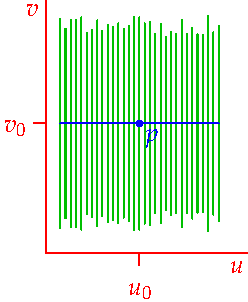
\includegraphics{adaptive-frobenius}
  \end{minipage}
  \item Finally, one shows that the resulting $\cE$ is differentiable with respect to $u$, and uses the compatibility condition to check that $\cE_u=\cE P$ as required.
\end{enumerate}
The first two steps may be accomplished approximately using a numerical method to desired accuracy, so this amounts to an algorithm for the approximation of $\cE$. The same approach can then be followed to approximate $\vx$.

 
\boldinline{The Gauss--Codazzi equations in curvature-line co-ordinates} Suppose we wish to define a surface with curvature-line co-ordinates $u,v$; we choose fundamental forms
\[\I=E\,\du^2+G\,\dv^2,\qquad \II=k_1E\,\du^2+k_2 G\dv^2\tag{$\dag$}\]
where $E,G$ are positive functions and $k_1,k_2$ the principal curvatures. It is sensible to choose metric forms $\theta_1=\sqrt E\,\du$ and $\theta_2=\sqrt G\,\dv$. In the language of Lemma \ref{lemm:gausspreq},
\[a=-k_1,\quad b=0,\quad c=-k_2,\quad \omega_{13}=-k_1\sqrt E\,\du,\quad\omega_{23}=-k_2\sqrt G\,\dv\]
The first structure equations determine (Exercise \ref{exs:gausscurvline})
\[\omega_{12}= \frac 1{2\sqrt{EG}}\left(E_v\,\du -G_u\,\dv\right)\]
The Gauss--Codazzi equations turn out to be equivalent to
\begin{align*}
\D\omega_{12}+\omega_{21}\wedge\omega_{13}=0\iff &\left(\frac{G_u}{\sqrt{EG}}\right)_u+\left(\frac{E_v}{\sqrt{EG}}\right)_v =-2k_1k_2\sqrt{EG}\\
\D\omega_{13}+\omega_{12}\wedge\omega_{23}=0\iff &2(k_1)_vE=(k_2-k_1)E_v\\
\D\omega_{23}+\omega_{21}\wedge\omega_{13}=0\iff &2(k_2)_uG=(k_1-k_2)G_u
\end{align*}
This makes it clear that there is an interdependence between $\I$ and $\II$: we cannot independently choose the metric and the curvatures. However, if $E,G,k_1,k_2$ satisfy these equations, Bonnet's theorem guarantees that there indeed exists a surface with fundamental forms $\dag$, unique up to rigid motions.\smallbreak
Even though $\I,\II$ cannot be chosen independently, Bonnet's result is still considered the best description of the \emph{minimal data} for a surface. You might suspect/hope that knowledge of $K,H$ would be enough to determine a surface up to rigid motions, but Exercise \ref{exs:tandevkh} shows such hope to be vain!

\goodbreak


\begin{exercises}{}{}
\exstart The unit cylinder $\vx(\phi,v)=\bigl(\cos\phi,\sin\phi,v\bigr)$ has adaptive frame
\[\ve_1=\threevec{-\sin\phi}{\cos\phi}{0},\qquad \ve_2=\threevec 001,\qquad \ve_3=\ve_1\times\ve_2=\threevec{\cos\phi}{\sin\phi}{0}\]
\begin{enumerate}\setcounter{enumi}{1}
  \item[]\begin{enumerate} 
    \item Directly compute the metric forms $\theta_j$ and connection forms $\omega_{jk}$.
    \item That the six structure equations are satisfied should be obvious from your answers to (a): why? 
    \item Why is it completely obvious from your answer to (a) that $K\equiv 0$?
  \end{enumerate}
  
  \item For a general regular surface, explain why we cannot, in general, find co-ordinates $u,v$ for which $\I=\du^2+\dv^2$.
  
  
  \item For the paraboloid example (\ref*{ex:adaptive}.\ref{exs:paraboloidconnectionform}) verify the Gauss--Codazzi equations $\D\lomega+\lomega\wedge\lomega=0$.\par
  (\emph{Hint: this is easier if you treat the three equations separately!}) 
  
  
  \item Verify that the metric $\I=\frac{\dx^2+\dy^2}{y^2}$ on the upper half-plane $y>0$ has curvature $K=-1$.\par
  (\emph{Hint: Recall Example \ref{ex:poincaredisc} and Exercise \ref*{sec:fund}.\ref{exs:poincarehalfplane}})
  

\item\label{exs:catenoidgauss} Consider the catenoid $\vx(u,v)=\bigl(\cos u\cosh v,\sin u\cosh v,v\bigr)$ obtained by revolving the catenary $x=\cosh z$ around the $z$-axis.
	\begin{enumerate}
	  \item Show that there exists a moving frame for which the metric forms are
	  \[\theta_1=\cosh v\,\du,\quad \theta_2=\cosh v\,\dv\]
	  \item Show that $\omega_{12}=\tanh v\,\du =\frac{\sinh v}{\cosh v}\,\du$ and use it to prove that the Gaussian curvature of the catenoid is
	  \[K=-\frac 1{\cosh^4v}\]
	\end{enumerate}
	
  
	\item We re-prove Exercise \ref*{sec:principalcurv}.\ref{exs:totallyumbilic} using our new language.
	\begin{enumerate}
	  \item Suppose a surface $\vx$ is totally umbilic: $\II=\lambda\I$, where $\lambda$ is some function. Explain why $\omega_{13}=-\lambda\theta_1$ and $\omega_{23}=-\lambda\theta_2$. 
	  \item Use the 1\st\ structure equations and the Codazzi equations to prove that $\D\lambda=0$.
		\item If $a=0$, what is $\vx$?
		\item If $a\neq 0$, define $\V c:=\vx-\frac 1a\ve_3$. Prove that $\D\V c=\V0$ and hence conclude that the surface is (part of a) round sphere.
	\end{enumerate}
	


  \item Suppose $\cE=\bigl(\ve_1\ \ve_2\ \ve_3\bigr)$ is an adaptive frame for a surface. Any other adaptive frame (with the same orientation) is obtained by \emph{rotating} around $\ve_3$: that is $\hat{\cE}=\bigl(\hat\ve_1\ \hat\ve_2\ \ve_3\bigr)$ where
  \[\hat\ve_1=\cos\varphi\,\ve_1+\sin\varphi\,\ve_2,\quad \hat\ve_2=-\sin\varphi\,\ve_1+\cos\varphi\,\ve_2\]
  for some smooth function $\varphi:U\to\R$.
  \begin{enumerate}
    \item Compute $\theta_1,\theta_2$ in terms of $\hat\theta_1,\hat\theta_2$ and conclude that $\hat\theta_1\wedge\hat\theta_2=\theta_1\wedge\theta_2$.
    \item Use Definition \ref{defn:mcforms} to compute $\hat\omega_{12}$ in terms of $\omega_{12}$ and $\varphi$. Verify that $\D\hat\omega_{12}=\D\omega_{12}$ so that the Gauss equation is identical for the new moving frame.
  \end{enumerate}
  

\goodbreak
  
  \item Suppose $\I$ is the 1\st\ fundamental form of a surface. Suppose $\I=\theta_1^2+\theta_2^2$ for some 1-forms $\theta_1,\theta_2$. Prove that there exists a moving frame $\cE=(\ve_1\ \ve_2\ \ve_3)$ for which $\dvx=\ve_1\theta_1+\ve_2\theta_2$.\par
  (\emph{Hint: consider the dual vector fields to $\theta_1,\theta_2$})
  
  
  \item\label{exs:gausscurvline} Suppose $u,v$ are orthogonal co-ordinates so that $\theta_1=\sqrt E\,\du$ and $\theta_2=\sqrt G\,\dv$.
  \begin{enumerate}
    \item Use the structure equations to prove that
    \[\omega_{12}= \frac 1{2\sqrt{EG}}\left(E_v\,\du -G_u\,\dv\right)\]
    \item Hence deduce an explicit formula for the Gauss curvature in terms of the coefficients of the 1\st\ fundamental form:
  	\[K=-\frac 1{2\sqrt{EG}}\left(\partials u\frac{G_u}{\sqrt{EG}}+\partials v\frac{E_v}{\sqrt{EG}}\right)\]
%   (\emph{Hint: let $\omega_{12}=f\,\du+g\,\dv$ and write $M=\sqrt E$ and $N=\sqrt G$ until the end of the calculation})
		\emph{This can be multiplied out to remove the square roots, though you'll get more terms. A nastier expression (the Brioshi formula) may be found for general co-ordinates with $F\neq 0$.}
		\end{enumerate}
  
  
  
  \item\label{exs:tandevkh} In Exercise \ref*{sec:principalcurv}.\ref{exs:tandevcurv} we saw that the tangent developable $\vx(u,v)=\vy(u)+v\vy'(u)$ of a unit-speed curve has curvatures $K=0$, $H=-\frac\tau{2v\kappa}$. Use this to describe \emph{two} surfaces with the same curvature functions which are not related by a direct isometry.
  
        
  \item Show that the surfaces parametrized by
  \[\vx(u,v)=\bigl(u\cos\phi,u\sin\phi,\ln u\bigr),\quad \vy(u,v)=\bigl(u\cos\phi,u\sin\phi,\phi\bigr)\]
  have the same Gauss curvature but distinct first fundamental forms $\I_\vx\neq\I_\vy$. To do this properly, you should argue that there is no reparametrization of $\vy$ so that $K_\vx=K_\vy$ and $\I_\vx=\I_\vy$.\par
  (\emph{Gauss' Theorem isn't bidirectional: surfaces can have the same $K$ without being locally isometric})
  
  
  \item Consider the family of surfaces
  \[\vx^t(u,v)=\cos t\threevec{\sin u\sinh v}{-\cos u\sinh v}{u}+ \sin t\threevec{\cos u\cosh v}{\sin u\cosh v}{v},\qquad t\in[0,\tfrac\pi 2]\]
   When $t=0$ this is a \emph{helicoid.} When $t=\frac\pi 2$ this is the \emph{catenoid} from Exercise \ref{exs:catenoidgauss}.
	\begin{enumerate}
  	\item Compute the first fundamental form of $\vx^t$ and show that it is independent of $t$ (the family $\vx^t$ is therefore \emph{isometric}). 
  	\item Show that the unit normal of $\vx^t$ is also independent of $t$:
 	 	\[\vn^t=\frac 1{\cosh v}\threevec{\cos u}{\sin u}{-\sinh v}\]
  	Hence compute the second fundamental form of $\vx^t$ for each $t$.
  	\item Find the Gauss and mean curvatures of all surfaces $\vx^t$. What is special about this family? Relate this to Gauss' Theorem.
\end{enumerate}

\end{enumerate}
\end{exercises}

\iffalse
\clearpage

GENERALIZE: IF $\vx:U\subseteq\R^m\to\E^n$ Define $\theta_1,\theta_2,\theta_3$ so that $\dvx=\sum_{j=1}^3\ve_j\theta_j$ and $\omega_{jk}$ as before.

\begin{examples}{}{}
Frenet frame: if $(m,n)=(1,3)$. If $\vx:U\to\E^3$ is a biregular curve, then $\dvx=\vx'(t)\,\dt$. If we take $(\ve_1\ \ve_2\ \ve_3)=(\vT\ \vN\ \vB)$ to be the Frenet frame, then the metric forms are
	\[\theta_1=\vT\cdot\dvx=v\,\dt,\quad \theta_2=\theta_3=0\]
	where $v$ is the speed of the curve. The Frenet--Serret equations show that
	\begin{gather*}
	\begin{aligned}
	\D E&=\bigl(\D\vT\ \D\vN\ \D\vB\bigr)=\bigl(\vT'\ \vN'\ \vB'\bigr)\dt =\bigl(\vT\ \vN\ \vB\bigr)
	\begin{pmatrix}
		0&-v\kappa&0\\
		v\kappa&0&-v\tau\\
		0&v\tau&0
	\end{pmatrix}\dt =E\lomega
	\end{aligned}
	\\
	\implies \omega_{12}=-v\kappa\,\dt,\quad \omega_{13}=0,\quad \omega_{23}=-v\tau\,\dt
	\end{gather*}
	Structure equations say nothing when $m=1$ since they are relations on 2-forms.

Cyl polar $(m,n)=(3,3)$. 
\end{examples}

 The structure equations are then

\begin{thm}{}{}
The metric and connection forms satisfy the \emph{first and second structure equations.} These can be stated either in matrix format, or multiplied out to three equivalent equations.
\begin{enumerate}
  \item $\D\Theta+\lomega\wedge\Theta=\V0\iff \D\theta_j+\sum\limits_{k\neq j}\omega_{jk}\wedge\theta_k=0$ for each $j=1,2,3$
  \item $\D\lomega+\lomega\wedge\lomega=0\iff \D\omega_{jk}+\omega_{ji}\wedge\omega_{ik}=0$ where $i,j,k$ are distinct.
\end{enumerate}
Writing these out explicitly, we obtain six equations: note the pattern in the indices!
\begin{align*}
&\D\theta_1+\omega_{12}\wedge\theta_2+\omega_{13}\wedge\theta_3=0 &&\D\omega_{12}+\omega_{13}\wedge\omega_{32}=0\\
&\D\theta_2+\omega_{21}\wedge\theta_1+\omega_{23}\wedge\theta_3=0 &&\D\omega_{13}+\omega_{12}\wedge\omega_{23}=0\\
&\D\theta_3+\omega_{31}\wedge\theta_1+\omega_{32}\wedge\theta_2=0 &&\D\omega_{23}+\omega_{21}\wedge\omega_{13}=0
\end{align*}
\end{thm}

GENERALIZE - optional section???? ($m=3$) \ For the cylindrical polar co-ordinate map $\vx(r,\psi,z)=\bigl(r\cos\psi,r\sin\psi,z\bigr)$, it would be sensible to choose a moving frame
	\[\textcolor{orange}{\ve_1}:=\partials[\vx]{r}=\threevec{\cos\psi}{\sin\psi}{0} \qquad \textcolor{blue}{\ve_2}:=r^{-1}\partials[\vx]{\psi}=\threevec{-\sin\psi}{\cos\psi}{0} \qquad \textcolor{Green}{\ve_3}=\partials[\vx]{z}=\threevec 001\]
	where the frame's axes point in the directions of change with respect to the three variables. %That these directions are orthogonal is a special property of cylindrical co-ordinates which is not true for general co-ordinate systems.
	For our cylindrical polar co-ordinate frame, we have
		\begin{gather*}
		\dvx=\vx_r\,\dr+\vx_\psi\,\D\psi+\vx_z\,\dz=\ve_1\,\dr+r\ve_2\,\D\psi+\ve_3\,\dz\\[5pt]
		\implies \theta_1=\dr,\ \ \theta_2=r\,\D\psi,\ \ \theta_3=\dz
		\end{gather*}
		 For cylindrical co-ordinates
	\begin{gather*}
	\D\ve_2=\threevec{-\cos\psi}{-\sin\psi}0\,\D\psi=-\ve_1\,\D\psi\implies \omega_{12}=-\D\psi,\quad\omega_{13}=0\\
	\D\ve_3=\V0\implies \omega_{23}=0
	\end{gather*}
	The connection form matrix is therefore $\lomega=\begin{smatrix}
	0&-1&0\\1&0&0\\0&0&0
	\end{smatrix}\D\psi$
	 These are a lot simpler:
	\begin{gather*}
	\D\Theta+\lomega\wedge\Theta =\threevec{0}{\dr\wedge\D\psi}{0} +\begin{pmatrix}
	0&-\D\psi&0\\\D\psi&0&0\\0&0&0
	\end{pmatrix}\wedge\threevec{\dr}{r\,\D\psi}{\dz}=\V0\\
	\D\lomega+\lomega\wedge\lomega =\begin{pmatrix}
	0&0&0\\0&0&0\\0&0&0
	\end{pmatrix}
	+
	\begin{pmatrix}
	0&-\D\psi&0\\\D\psi&0&0\\0&0&0
	\end{pmatrix}
	\wedge
	\begin{pmatrix}
	0&-\D\psi&0\\\D\psi&0&0\\0&0&0
	\end{pmatrix}
	=0
	\end{gather*}
	
	\href{http://www.math.uci.edu/~ndonalds/math162a/moving-cylinder.html}{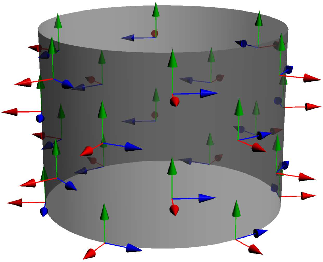
\includegraphics{moving-cylinder}}

EXERCISE - check that metric forms determine connection forms for cyl polars!
It is straightforward to see the forms for our cylindrical co-ordinate example satisfy both structure equations. It is less easy to see that the $\omega_{ij}$ are in fact determined by the structure equations and the $\theta_i$. In this example we have,
\[\theta_1=\D r,\quad \theta_2=r\D\phi,\quad \theta_3=\D z,\quad \D\theta_1=\D\theta_3=0,\quad \D\theta_2=\D r\wedge\D\phi.\]
The first structure equations then give us,
\[\left.\begin{array}{l} 
\D\theta_1=0=-\omega_{12}\wedge r\D\phi-\omega_{13}\wedge\D z\\ 
\D\theta_2=\D r\wedge\D\phi=\omega_{12}\wedge\D r-\omega_{23}\wedge\D z\\ 
\D\theta_3=0=\omega_{13}\wedge\D r+\omega_{23}\wedge r\D\phi 
\end{array}\right\}.\]
A little thought leads us through the following:
\begin{itemize}
  \item $\omega_{13}$ is a combination of $\D\phi$ and $\dz$ by the first equation, and of $\D r$ and $\D\phi$ by the third. Since $\D r,\D\phi,\dz$ are linearly independent at each point we must have $\omega_{13}$ a multiple of $\D\phi$ only. Write $\omega_{13}=ra\D\phi$ for some function $a$.
  \item The first and third equations now say that $\omega_{12}=b\D\phi+a\D z$, $\omega_{23}=a\D r+c\D\phi$, for some functions $b,c$.
  \item Plugging all this into the second equation yields
  \begin{gather*}
  \D r\wedge\D\phi=b\D\phi\wedge\D r+a\dz\wedge\D r-a\D r\wedge\D z-c\D\phi\wedge\dz,\\
  \therefore (1+b)\D r\wedge\D\phi+2a\D r\wedge\dz+c\D\phi\wedge\dz=0.
  \end{gather*}
  \item The linear independence of the above three 2-forms at each point guarantees that all coefficients are zero so that $a=c=0$ and $b=-1$, thus recovering $\omega_{ij}$.
\end{itemize}


The point of the above exercise is to see that the connection 1-forms of a moving frame are generally determined directly by the forms $\theta_i$. In practical examples (surfaces later for instance), the $\theta_i$'s are synonymous with the induced metric of the surface. This method of imposing a metric (choice of first fundamental form), and calculating the connection 1-forms from it is critical in physical applications --- we shall do a little of this later. It will be seen that the Gauss curvature of a surface can be calculated directly from the connection 1-forms. The generalization of this to higher dimensions is the method by which the \emph{Riemann curvature tensor} of the (Levi--Civita) \emph{connection} of a metric is calculated. Indeed the relationship between a surface/manifold, metric, connection and Gauss/Riemann curvature is precisely what Physicists are talking about when they say that `Spacetime is curved'.


\begin{exercises}{}{}
\begin{enumerate}
  \item 


 
  
  \item\begin{enumerate}
     \item We have defined Gauss and mean curvature for orientable (local) surfaces. Define the Gaussian curvature of a non-orientable surface and explain why the mean curvature of a non-orientable surface is not well-defined.
     \item The map
\[\vx(u,v)=\threevec{(2-v\sin(u/2))\sin u}{(2-v\sin(u/2))\cos u}{v\cos(u/2)},\]
defines a Möbius strip in $\E^3$. Show directly that $\vx$ is non-orientable, and that its Gaussian curvature is
\[K=-\frac{1}{(v^2/4+(2-v\sin(u/2))^2)^2}.\]
\begin{center}
%\includegraphics[width=0.5\textwidth]{Mobius1} \qquad \includegraphics[width=0.33\textwidth]{Mobius2}
\end{center}
        \end{enumerate}

\end{enumerate}
\end{exercises}


% \subsection{Conjugate directions, line congruences and focal surfaces}
% 
% This final section is a fun link between geometry and classical PDE theory. It starts from a related concept to asymptotic directions.
% 
% \begin{defn}
% Two tangent vectors $v,w\in T_pU$ are \emph{conjugate} for a surface $\vx$, if $\II(v,w)=0$. Co-ordinates $x,y$ on $U$ are conjugate if the co-ordinate vector fields $\partials x,\partials y$ are conjugate directions in every tangent space $T_pU$.
% \end{defn}
% 
% Asymptotic directions are thus conjugate to themselves.
% 
% The following proposition is tautological.
% 
% \begin{prop}
% Co-ordinates $u,v$ are conjugate for a surface $\vx$ iff there exist function $a,b$ such that $\vx_{uv}+a\vx_u+b\vx_v=0$.
% \end{prop}
% 
% Each of the entries (with respect to some basis) of the parameterized surface $\vx$ are solutions of the differential equation $f_{uv}+af_u+bf_v=0$. This is a hyperbolic equation and there exists no general way of solving these. However, the link with geometry gives a method of transforming solutions into new solutions to related equation. Here's how.
% 
% \begin{defn}
% Let $\vx:U\to\E^3$ be a surface and let $X$ be a vector field on $U$. Then
% \[\vy:=\vx+\dvx(X)\]
% is a new surface, obtained by walking off the surface $\vx$ in a tangent direction a distance depending on $X$. We say that $\vx$ is a \emph{focal surface} for the family of lines $L:\vx\to\E^3:s\mapsto\{\vx(s)+t\dvx_s(\at Xs):t\in\R\}$. We call $L$
%  a \emph{line congruence}.
% \end{defn}
%  
% Suppose that $u,v$ are conjugate co-ordinates for $\vx$. For each $\lambda\in\R$, consider the function $\vy_\lambda:U\to\E^3$ defined by
% \[\vy_\lambda=\vx+\lambda\vx_u.\]
% The set of lines joining $\vx$ and $\vy_\lambda$ (for any $\lambda\neq 0$) form a line congruence.
% 
% \begin{prop}
% $\vy_\lambda$ is a focal surface for the above line congruence iff $\lambda=0$ or $a$.
% \end{prop}
% 
% \begin{proof}
% $\vy_\lambda$ is a focal surface for the congruence joining $\vx,\vy_\lambda$ iff there exist functions $e,f$ such that $\vy_\lambda+e\vy_\lambda+f\vy_\lambda=\vx$.
% \end{proof}
% 
% The set of lines $\{L_t:\vx+t(\vy-\vx)\}$ is a line congruence for which $\vx$ is focal. We want to see when $\vy$ is also focal for the congruence. That is we want functions $m$ such that
% \[\vy+m\vy_v=\vx.\]
% Solving this we have
% \[\vx=\vx+k\vx_u+m(\vx_v+k_v\vx_u+k\vx_{uv})=\vx+(k+k_vm+am)\vx_u+m(1+kb)\vx_v.\]
% Yuk. Just do with conjugate to start with.


\fi